% Seminar 13: Machine learning
% Statistics of Financial Markets -- Bachelor's programme, Bucharest University of Economic Studies
% GENERATED by latex/build_seminar13.py -- edit the generator, not this file.
% Student version by default; the instructor version is the *_solutions.tex wrapper.
\makeatletter\@ifundefined{ifsolutions}{\expandafter\newif\csname ifsolutions\endcsname}{}\makeatother

\newcommand{\coursename}{Statistics of Financial Markets}
% Preambul comun SFM -- Statistica piețelor financiare / Statistics of Financial Markets (Beamer, 16:9)
% Același design ca MFM. Înainte de % Preambul comun SFM -- Statistica piețelor financiare / Statistics of Financial Markets (Beamer, 16:9)
% Același design ca MFM. Înainte de % Preambul comun SFM -- Statistica piețelor financiare / Statistics of Financial Markets (Beamer, 16:9)
% Același design ca MFM. Înainte de \input{../../latex/preamble} se definește
%   \newcommand{\coursename}{Statistics of Financial Markets}      (EN)
%   \newcommand{\coursename}{Statistica piețelor financiare}       (RO)  și  \def\sfmlang{ro}
% Fișierele .tex se află în EN/Courses, EN/Seminars, RO/Cursuri, RO/Seminarii (două niveluri sub rădăcină).
% Deck-urile sînt generate de latex/build_chapterN.py / build_seminarN.py (vezi latex/sfm_build.py).

\documentclass[9pt, aspectratio=169, t]{beamer}
\providecommand{\coursename}{Statistics of Financial Markets}

% Ensure content fits on slides
\setbeamersize{text margin left=8mm, text margin right=8mm}

%=============================================================================
% THEME AND STYLE CONFIGURATION
%=============================================================================
\usetheme{default}
% Using default theme for clean header/footer control

% Color Palette (matching Redispatch PDF)
\definecolor{MainBlue}{RGB}{26, 58, 110}
\definecolor{AccentBlue}{RGB}{26, 58, 110}
\definecolor{IDAred}{RGB}{205, 0, 0}
\definecolor{DarkGray}{RGB}{51, 51, 51}
\definecolor{MediumGray}{RGB}{128, 128, 128}
\definecolor{LightGray}{RGB}{248, 248, 248}
\definecolor{VeryLightGray}{RGB}{235, 235, 235}
\definecolor{KeynoteGray}{RGB}{218, 218, 218}
\definecolor{SectionGray}{RGB}{120, 120, 120}
\definecolor{FooterGray}{RGB}{100, 100, 100}
\definecolor{Crimson}{RGB}{220, 53, 69}
\definecolor{Forest}{RGB}{46, 125, 50}
\definecolor{Amber}{RGB}{181, 133, 63}
\definecolor{Orange}{RGB}{230, 126, 34}
\definecolor{Purple}{RGB}{142, 68, 173}

% Gradient background (exact Keynote 315° gradient: white to RGB 218,218,218)
\setbeamertemplate{background}{%
    \begin{tikzpicture}[remember picture, overlay]
        \shade[shading=axis, shading angle=315,
        top color=white, bottom color=KeynoteGray]
        (current page.south west) rectangle (current page.north east);
    \end{tikzpicture}%
}
% Fallback solid color for compatibility
\setbeamercolor{background canvas}{bg=}

\setbeamercolor{palette primary}{bg=MainBlue, fg=white}
\setbeamercolor{palette secondary}{bg=MainBlue!85, fg=white}
\setbeamercolor{palette tertiary}{bg=MainBlue!70, fg=white}
\setbeamercolor{structure}{fg=MainBlue}
\setbeamercolor{title}{fg=IDAred}
\setbeamercolor{frametitle}{fg=IDAred, bg=}
\setbeamercolor{block title}{bg=MainBlue, fg=white}
\setbeamercolor{block body}{bg=VeryLightGray, fg=DarkGray}
\setbeamercolor{block title alerted}{bg=Crimson, fg=white}
\setbeamercolor{block body alerted}{bg=Crimson!8, fg=DarkGray}
\setbeamercolor{block title example}{bg=Forest, fg=white}
\setbeamercolor{block body example}{bg=Forest!8, fg=DarkGray}
\setbeamercolor{item}{fg=MainBlue}

% Footer colors (override Madrid theme blue)
\setbeamercolor{author in head/foot}{fg=FooterGray, bg=}
\setbeamercolor{title in head/foot}{fg=FooterGray, bg=}
\setbeamercolor{date in head/foot}{fg=FooterGray, bg=}
\setbeamercolor{section in head/foot}{fg=FooterGray, bg=}
\setbeamercolor{subsection in head/foot}{fg=FooterGray, bg=}

% Bullet styles (apply everywhere including blocks)
\setbeamertemplate{itemize item}{\color{MainBlue}$\boxdot$}
\setbeamertemplate{itemize subitem}{\color{MainBlue}$\blacktriangleright$}
\setbeamertemplate{itemize subsubitem}{\color{MainBlue}\tiny$\bullet$}
\setbeamertemplate{itemize/enumerate body begin}{\normalsize}
\setbeamertemplate{itemize/enumerate subbody begin}{\normalsize}

% Item spacing - compact style
\setlength{\leftmargini}{10pt}       % Level 1: minimal indent
\setlength{\leftmarginii}{10pt}      % Level 2: minimal additional indent
% Compact list spacing (zero extra space before/after lists in blocks)
\makeatletter
\def\@listi{\leftmargin\leftmargini \topsep 0pt \parsep 0pt \itemsep 0pt}
\def\@listii{\leftmargin\leftmarginii \topsep 0pt \parsep 0pt \itemsep 0pt}
\makeatother

\setbeamertemplate{navigation symbols}{}

%=============================================================================
% CUSTOM HEADLINE
%=============================================================================
\setbeamertemplate{headline}{%
    \vskip10pt%
    \hbox to \paperwidth{%
        \hskip0.5cm%
        {\small\color{FooterGray}\renewcommand{\hyperlink}[2]{##2}\insertsectionhead}%
        \hfill%
        \textcolor{FooterGray}{\small\insertframenumber}%
        \hskip0.5cm%
    }%
    \vskip4pt%
    {\color{FooterGray}\hrule height 0.4pt}%
}

%=============================================================================
% CUSTOM FOOTER
%=============================================================================
\usepackage{fontawesome5}

\setbeamertemplate{footline}{%
    {\color{FooterGray}\hrule height 0.4pt}%
    \vskip4pt%
    \hbox to \paperwidth{%
        \hskip0.5cm%
        \textcolor{FooterGray}{\small\coursename}%
        \hfill%
        \raisebox{-0.1em}{%
            \begin{tikzpicture}[x=0.08em, y=0.08em, line width=0.4pt]
                \draw[FooterGray] (0,3) -- (1,4) -- (2,3.5) -- (3,5) -- (4,4) -- (5,6) -- (6,5.5) -- (7,4) -- (8,5) -- (9,7) -- (10,6) -- (11,5) -- (12,6.5) -- (13,8) -- (14,7) -- (15,6) -- (16,7.5) -- (17,9) -- (18,8) -- (19,7) -- (20,8.5) -- (21,10) -- (22,9) -- (23,8) -- (24,9.5);
            \end{tikzpicture}%
        }%
        \hskip0.5cm%
    }%
    \vskip6pt%
}

%=============================================================================
% PACKAGES
%=============================================================================
\usepackage[utf8]{inputenc}
\DeclareUnicodeCharacter{03B1}{\ensuremath{\alpha}}
\usepackage[T1]{fontenc}
\usepackage{amsmath, amssymb, amsthm}
\usepackage{mathtools}
\usepackage{bm}
\usepackage{tikz}
\usetikzlibrary{arrows.meta, positioning, shapes, calc, decorations.pathreplacing, shadings}
\usepackage{booktabs}
\usepackage{multirow}
\usepackage{array}
\usepackage{graphicx}
\usepackage{hyperref}
\usepackage{colortbl}
\usepackage{listings}
\lstset{language=Python, basicstyle=\ttfamily\scriptsize, keywordstyle=\color{MainBlue}\bfseries,
  commentstyle=\color{Forest}, stringstyle=\color{Crimson}, breaklines=true,
  frame=none, backgroundcolor=\color{VeryLightGray}, xleftmargin=2mm}
\hypersetup{colorlinks=true, linkcolor=MainBlue, urlcolor=MainBlue}
\graphicspath{{../../logos/}{../../charts/}{../../photos/}}
\usepackage{xcolor}
\hfuzz=2pt  % Suppress tiny overfull warnings (<2pt)
\vfuzz=2pt  % Suppress tiny vertical overfull warnings (<2pt)

%=============================================================================
% QUANTLET COMMANDS
%   \quantlet{<displayed name>}{<url>}       (generic, compatible with the older SFM decks)
%   \sfmquantlet{Ch_05}{SFM_ch5_garch}       -> https://github.com/danpele/SFM/tree/main/Quantlets/Ch_05/SFM_ch5_garch
%   \qlurl{<folder>} is defined per chapter by the generator (Quantlets/Ch_NN/<folder>)
%=============================================================================
\newcommand{\sfmrepo}{https://github.com/danpele/SFM}
\newcommand{\sfmqlbase}{https://github.com/danpele/SFM/tree/main/Quantlets}
\newcommand{\quantlet}[2]{%
    \hfill\href{#2}{%
        \raisebox{-0.15em}{
\includegraphics[height=0.7em]{ql_logo.png}}%
        \textcolor{MainBlue}{\tiny\ #1}%
    }%
}
\newcommand{\sfmquantlet}[2]{\quantlet{\detokenize{#2}}{\sfmqlbase/#1/#2}}

%=============================================================================
% NOTEBOOKS (Google Colab)
%   \colaburl{notebooks/EN/chapter5_seminar_notebook.ipynb} -> the Colab link of a file in the SFM repo
%   \nb: the chapter notebook (each seminar deck redefines it with \renewcommand)
%=============================================================================
\newcommand{\colaburl}[1]{https://colab.research.google.com/github/danpele/SFM/blob/main/#1}
\newcommand{\nb}{https://colab.research.google.com/github/danpele/SFM/tree/main/notebooks/EN}
\newcommand{\nbname}{notebooks/EN}

%=============================================================================
% SLIDE HELPERS (used by the generators; the same as in MFM)
%=============================================================================
% local font size for list bodies (the preamble forces \normalsize)
\newcommand{\itemsize}[1]{\setbeamertemplate{itemize/enumerate body begin}{#1}\setbeamertemplate{itemize/enumerate subbody begin}{#1}}
\newcommand{\intitle}[1]{{\hypersetup{urlcolor=white}#1}}   % white links inside coloured title bars
\newcommand{\imgcap}[1]{{\scriptsize #1}\\[0.5mm]}          % caption under a photo
\newcommand{\imgcredit}[2]{{\tiny\color{FooterGray}\href{#1}{#2}}}   % image credit: source URL, author/licence
\newcommand{\aiprompt}[1]{{\ttfamily\color{MainBlue}#1}}     % a prompt to an AI assistant

%=============================================================================
% SEMINARS: student version by default; the instructor wrapper *_solutions.tex sets \solutionstrue
%=============================================================================
\makeatletter\@ifundefined{ifsolutions}{\expandafter\newif\csname ifsolutions\endcsname}{}\makeatother
\newcommand{\solonly}[1]{\ifsolutions #1\fi}
\newcommand{\propsub}{\ifsolutions\else\framesubtitle{\ifdefined\sfmlang Rezolvarea se discută la seminar\else Solution discussed in class\fi}\fi}

%=============================================================================
% APPENDIX AND CHAPTER LINKS (latex/appendix_links.py writes the calls; it also re-declares these
% macros before \begin{document}, so the decks compile with or without this preamble block)
%=============================================================================
\providecommand{\sfmapplink}[3]{\hypertarget{#2}{}\hyperlink{#1}{\beamergotobutton{#3}}}
\providecommand{\sfmappback}[2]{\begin{tikzpicture}[remember picture,overlay]\node[anchor=south east] at ([xshift=-3mm,yshift=7mm]current page.south east){\hyperlink{#1}{\beamerreturnbutton{#2}}};\end{tikzpicture}}
\providecommand{\sfmchlink}[2]{\href{#1}{#2}}
\providecommand{\sfmchlinkt}[2]{\href{#1}{\usebeamercolor[fg]{frametitle}#2}}

%=============================================================================
% QUANTINAR COMMAND: link către un curs Quantinar (subiecte avansate)
%=============================================================================
\newcommand{\quantinar}[2]{%
    \href{#2}{%
        \raisebox{-0.15em}{
\includegraphics[height=0.8em]{qr_logo.png}}%
        \textcolor{MainBlue}{\scriptsize\ #1}%
    }%
}

%=============================================================================
% CUSTOM TITLE PAGE
%=============================================================================
\defbeamertemplate*{title page}{hybrid}[1][]
{
    \vspace{0.2cm}
    % Logos row - top header (with clickable links)
    \begin{center}
        \href{https://www.ase.ro}{
\includegraphics[height=1.0cm]{ase_logo.png}}\hspace{0.3cm}%
        \href{https://theida.net}{
\includegraphics[height=1.0cm]{ida_logo.png}}\hspace{0.3cm}%
        \href{https://blockchain-research-center.com}{
\includegraphics[height=1.0cm]{brc_logo.png}}\hspace{0.3cm}%
        \href{https://www.ai4efin.ase.ro}{
\includegraphics[height=1.0cm]{ai4efin_logo.png}}\hspace{0.3cm}%
        \href{https://ipe.ro/new}{
\includegraphics[height=1.0cm]{acad_logo.png}}\hspace{0.3cm}%
        \href{https://www.digital-finance-msca.com}{
\includegraphics[height=1.0cm]{msca_logo.png}}%
    \end{center}

    \vspace{0.6cm}

    % Main title with Q logos on sides (with clickable links)
    \begin{center}
        \begin{minipage}{0.1\textwidth}
            \centering
            \href{https://quantlet.com}{
\includegraphics[height=1.1cm]{ql_logo.png}}
        \end{minipage}%
        \begin{minipage}{0.78\textwidth}
            \centering
            {\LARGE\bfseries\usebeamercolor[fg]{title}\inserttitle}

            \vspace{0.3cm}

            {\usebeamerfont{subtitle}\usebeamercolor[fg]{title}\insertsubtitle}
        \end{minipage}%
        \begin{minipage}{0.1\textwidth}
            \centering
            \href{https://quantinar.com}{
\includegraphics[height=1.1cm]{qr_logo.png}}
        \end{minipage}
    \end{center}

    \vspace{0.6cm}

    % Authors (left aligned)
    \hspace{0.5cm}{\usebeamerfont{author}\insertauthor}

    \vspace{0.3cm}

    % Institute/Affiliations (left aligned)
    \hspace{0.5cm}\begin{minipage}[t]{0.9\textwidth}
        \raggedright\small\insertinstitute
    \end{minipage}
}

%=============================================================================
% THEOREM ENVIRONMENTS
%=============================================================================
\theoremstyle{definition}
\setbeamertemplate{theorems}[numbered]
\ifdefined\sfmlang
\newtheorem{defn}{Definiție}
\newtheorem{thm}{Teoremă}
\newtheorem{prop}{Propoziție}
\newtheorem{rmk}{Observație}
\else
\newtheorem{defn}{Definition}
\newtheorem{thm}{Theorem}
\newtheorem{prop}{Proposition}
\newtheorem{rmk}{Remark}
\fi

%=============================================================================
% CENTRED MINIPAGE (no extra vertical space)
%=============================================================================
\newenvironment{cminipage}[1]{%
    \par\noindent\hfill\begin{minipage}{#1}\ignorespaces
}{%
    \end{minipage}\hfill\null\par
}

%=============================================================================
% CUSTOM COMMANDS
%=============================================================================
\newcommand{\E}{\mathbb{E}}
\newcommand{\Var}{\text{Var}}
\newcommand{\Cov}{\text{Cov}}
\newcommand{\Corr}{\text{Corr}}
\newcommand{\R}{\mathbb{R}}
\newcommand{\N}{\mathbb{N}}
\newcommand{\Z}{\mathbb{Z}}
\newcommand{\B}{\mathbf{B}}
\newcommand{\imark}{\textcolor{MainBlue}{\textbullet}}
\newcommand{\RMSE}{\text{RMSE}}
\newcommand{\MAE}{\text{MAE}}
\newcommand{\MAPE}{\text{MAPE}}

 se definește
%   \newcommand{\coursename}{Statistics of Financial Markets}      (EN)
%   \newcommand{\coursename}{Statistica piețelor financiare}       (RO)  și  \def\sfmlang{ro}
% Fișierele .tex se află în EN/Courses, EN/Seminars, RO/Cursuri, RO/Seminarii (două niveluri sub rădăcină).
% Deck-urile sînt generate de latex/build_chapterN.py / build_seminarN.py (vezi latex/sfm_build.py).

\documentclass[9pt, aspectratio=169, t]{beamer}
\providecommand{\coursename}{Statistics of Financial Markets}

% Ensure content fits on slides
\setbeamersize{text margin left=8mm, text margin right=8mm}

%=============================================================================
% THEME AND STYLE CONFIGURATION
%=============================================================================
\usetheme{default}
% Using default theme for clean header/footer control

% Color Palette (matching Redispatch PDF)
\definecolor{MainBlue}{RGB}{26, 58, 110}
\definecolor{AccentBlue}{RGB}{26, 58, 110}
\definecolor{IDAred}{RGB}{205, 0, 0}
\definecolor{DarkGray}{RGB}{51, 51, 51}
\definecolor{MediumGray}{RGB}{128, 128, 128}
\definecolor{LightGray}{RGB}{248, 248, 248}
\definecolor{VeryLightGray}{RGB}{235, 235, 235}
\definecolor{KeynoteGray}{RGB}{218, 218, 218}
\definecolor{SectionGray}{RGB}{120, 120, 120}
\definecolor{FooterGray}{RGB}{100, 100, 100}
\definecolor{Crimson}{RGB}{220, 53, 69}
\definecolor{Forest}{RGB}{46, 125, 50}
\definecolor{Amber}{RGB}{181, 133, 63}
\definecolor{Orange}{RGB}{230, 126, 34}
\definecolor{Purple}{RGB}{142, 68, 173}

% Gradient background (exact Keynote 315° gradient: white to RGB 218,218,218)
\setbeamertemplate{background}{%
    \begin{tikzpicture}[remember picture, overlay]
        \shade[shading=axis, shading angle=315,
        top color=white, bottom color=KeynoteGray]
        (current page.south west) rectangle (current page.north east);
    \end{tikzpicture}%
}
% Fallback solid color for compatibility
\setbeamercolor{background canvas}{bg=}

\setbeamercolor{palette primary}{bg=MainBlue, fg=white}
\setbeamercolor{palette secondary}{bg=MainBlue!85, fg=white}
\setbeamercolor{palette tertiary}{bg=MainBlue!70, fg=white}
\setbeamercolor{structure}{fg=MainBlue}
\setbeamercolor{title}{fg=IDAred}
\setbeamercolor{frametitle}{fg=IDAred, bg=}
\setbeamercolor{block title}{bg=MainBlue, fg=white}
\setbeamercolor{block body}{bg=VeryLightGray, fg=DarkGray}
\setbeamercolor{block title alerted}{bg=Crimson, fg=white}
\setbeamercolor{block body alerted}{bg=Crimson!8, fg=DarkGray}
\setbeamercolor{block title example}{bg=Forest, fg=white}
\setbeamercolor{block body example}{bg=Forest!8, fg=DarkGray}
\setbeamercolor{item}{fg=MainBlue}

% Footer colors (override Madrid theme blue)
\setbeamercolor{author in head/foot}{fg=FooterGray, bg=}
\setbeamercolor{title in head/foot}{fg=FooterGray, bg=}
\setbeamercolor{date in head/foot}{fg=FooterGray, bg=}
\setbeamercolor{section in head/foot}{fg=FooterGray, bg=}
\setbeamercolor{subsection in head/foot}{fg=FooterGray, bg=}

% Bullet styles (apply everywhere including blocks)
\setbeamertemplate{itemize item}{\color{MainBlue}$\boxdot$}
\setbeamertemplate{itemize subitem}{\color{MainBlue}$\blacktriangleright$}
\setbeamertemplate{itemize subsubitem}{\color{MainBlue}\tiny$\bullet$}
\setbeamertemplate{itemize/enumerate body begin}{\normalsize}
\setbeamertemplate{itemize/enumerate subbody begin}{\normalsize}

% Item spacing - compact style
\setlength{\leftmargini}{10pt}       % Level 1: minimal indent
\setlength{\leftmarginii}{10pt}      % Level 2: minimal additional indent
% Compact list spacing (zero extra space before/after lists in blocks)
\makeatletter
\def\@listi{\leftmargin\leftmargini \topsep 0pt \parsep 0pt \itemsep 0pt}
\def\@listii{\leftmargin\leftmarginii \topsep 0pt \parsep 0pt \itemsep 0pt}
\makeatother

\setbeamertemplate{navigation symbols}{}

%=============================================================================
% CUSTOM HEADLINE
%=============================================================================
\setbeamertemplate{headline}{%
    \vskip10pt%
    \hbox to \paperwidth{%
        \hskip0.5cm%
        {\small\color{FooterGray}\renewcommand{\hyperlink}[2]{##2}\insertsectionhead}%
        \hfill%
        \textcolor{FooterGray}{\small\insertframenumber}%
        \hskip0.5cm%
    }%
    \vskip4pt%
    {\color{FooterGray}\hrule height 0.4pt}%
}

%=============================================================================
% CUSTOM FOOTER
%=============================================================================
\usepackage{fontawesome5}

\setbeamertemplate{footline}{%
    {\color{FooterGray}\hrule height 0.4pt}%
    \vskip4pt%
    \hbox to \paperwidth{%
        \hskip0.5cm%
        \textcolor{FooterGray}{\small\coursename}%
        \hfill%
        \raisebox{-0.1em}{%
            \begin{tikzpicture}[x=0.08em, y=0.08em, line width=0.4pt]
                \draw[FooterGray] (0,3) -- (1,4) -- (2,3.5) -- (3,5) -- (4,4) -- (5,6) -- (6,5.5) -- (7,4) -- (8,5) -- (9,7) -- (10,6) -- (11,5) -- (12,6.5) -- (13,8) -- (14,7) -- (15,6) -- (16,7.5) -- (17,9) -- (18,8) -- (19,7) -- (20,8.5) -- (21,10) -- (22,9) -- (23,8) -- (24,9.5);
            \end{tikzpicture}%
        }%
        \hskip0.5cm%
    }%
    \vskip6pt%
}

%=============================================================================
% PACKAGES
%=============================================================================
\usepackage[utf8]{inputenc}
\DeclareUnicodeCharacter{03B1}{\ensuremath{\alpha}}
\usepackage[T1]{fontenc}
\usepackage{amsmath, amssymb, amsthm}
\usepackage{mathtools}
\usepackage{bm}
\usepackage{tikz}
\usetikzlibrary{arrows.meta, positioning, shapes, calc, decorations.pathreplacing, shadings}
\usepackage{booktabs}
\usepackage{multirow}
\usepackage{array}
\usepackage{graphicx}
\usepackage{hyperref}
\usepackage{colortbl}
\usepackage{listings}
\lstset{language=Python, basicstyle=\ttfamily\scriptsize, keywordstyle=\color{MainBlue}\bfseries,
  commentstyle=\color{Forest}, stringstyle=\color{Crimson}, breaklines=true,
  frame=none, backgroundcolor=\color{VeryLightGray}, xleftmargin=2mm}
\hypersetup{colorlinks=true, linkcolor=MainBlue, urlcolor=MainBlue}
\graphicspath{{../../logos/}{../../charts/}{../../photos/}}
\usepackage{xcolor}
\hfuzz=2pt  % Suppress tiny overfull warnings (<2pt)
\vfuzz=2pt  % Suppress tiny vertical overfull warnings (<2pt)

%=============================================================================
% QUANTLET COMMANDS
%   \quantlet{<displayed name>}{<url>}       (generic, compatible with the older SFM decks)
%   \sfmquantlet{Ch_05}{SFM_ch5_garch}       -> https://github.com/danpele/SFM/tree/main/Quantlets/Ch_05/SFM_ch5_garch
%   \qlurl{<folder>} is defined per chapter by the generator (Quantlets/Ch_NN/<folder>)
%=============================================================================
\newcommand{\sfmrepo}{https://github.com/danpele/SFM}
\newcommand{\sfmqlbase}{https://github.com/danpele/SFM/tree/main/Quantlets}
\newcommand{\quantlet}[2]{%
    \hfill\href{#2}{%
        \raisebox{-0.15em}{
\includegraphics[height=0.7em]{ql_logo.png}}%
        \textcolor{MainBlue}{\tiny\ #1}%
    }%
}
\newcommand{\sfmquantlet}[2]{\quantlet{\detokenize{#2}}{\sfmqlbase/#1/#2}}

%=============================================================================
% NOTEBOOKS (Google Colab)
%   \colaburl{notebooks/EN/chapter5_seminar_notebook.ipynb} -> the Colab link of a file in the SFM repo
%   \nb: the chapter notebook (each seminar deck redefines it with \renewcommand)
%=============================================================================
\newcommand{\colaburl}[1]{https://colab.research.google.com/github/danpele/SFM/blob/main/#1}
\newcommand{\nb}{https://colab.research.google.com/github/danpele/SFM/tree/main/notebooks/EN}
\newcommand{\nbname}{notebooks/EN}

%=============================================================================
% SLIDE HELPERS (used by the generators; the same as in MFM)
%=============================================================================
% local font size for list bodies (the preamble forces \normalsize)
\newcommand{\itemsize}[1]{\setbeamertemplate{itemize/enumerate body begin}{#1}\setbeamertemplate{itemize/enumerate subbody begin}{#1}}
\newcommand{\intitle}[1]{{\hypersetup{urlcolor=white}#1}}   % white links inside coloured title bars
\newcommand{\imgcap}[1]{{\scriptsize #1}\\[0.5mm]}          % caption under a photo
\newcommand{\imgcredit}[2]{{\tiny\color{FooterGray}\href{#1}{#2}}}   % image credit: source URL, author/licence
\newcommand{\aiprompt}[1]{{\ttfamily\color{MainBlue}#1}}     % a prompt to an AI assistant

%=============================================================================
% SEMINARS: student version by default; the instructor wrapper *_solutions.tex sets \solutionstrue
%=============================================================================
\makeatletter\@ifundefined{ifsolutions}{\expandafter\newif\csname ifsolutions\endcsname}{}\makeatother
\newcommand{\solonly}[1]{\ifsolutions #1\fi}
\newcommand{\propsub}{\ifsolutions\else\framesubtitle{\ifdefined\sfmlang Rezolvarea se discută la seminar\else Solution discussed in class\fi}\fi}

%=============================================================================
% APPENDIX AND CHAPTER LINKS (latex/appendix_links.py writes the calls; it also re-declares these
% macros before \begin{document}, so the decks compile with or without this preamble block)
%=============================================================================
\providecommand{\sfmapplink}[3]{\hypertarget{#2}{}\hyperlink{#1}{\beamergotobutton{#3}}}
\providecommand{\sfmappback}[2]{\begin{tikzpicture}[remember picture,overlay]\node[anchor=south east] at ([xshift=-3mm,yshift=7mm]current page.south east){\hyperlink{#1}{\beamerreturnbutton{#2}}};\end{tikzpicture}}
\providecommand{\sfmchlink}[2]{\href{#1}{#2}}
\providecommand{\sfmchlinkt}[2]{\href{#1}{\usebeamercolor[fg]{frametitle}#2}}

%=============================================================================
% QUANTINAR COMMAND: link către un curs Quantinar (subiecte avansate)
%=============================================================================
\newcommand{\quantinar}[2]{%
    \href{#2}{%
        \raisebox{-0.15em}{
\includegraphics[height=0.8em]{qr_logo.png}}%
        \textcolor{MainBlue}{\scriptsize\ #1}%
    }%
}

%=============================================================================
% CUSTOM TITLE PAGE
%=============================================================================
\defbeamertemplate*{title page}{hybrid}[1][]
{
    \vspace{0.2cm}
    % Logos row - top header (with clickable links)
    \begin{center}
        \href{https://www.ase.ro}{
\includegraphics[height=1.0cm]{ase_logo.png}}\hspace{0.3cm}%
        \href{https://theida.net}{
\includegraphics[height=1.0cm]{ida_logo.png}}\hspace{0.3cm}%
        \href{https://blockchain-research-center.com}{
\includegraphics[height=1.0cm]{brc_logo.png}}\hspace{0.3cm}%
        \href{https://www.ai4efin.ase.ro}{
\includegraphics[height=1.0cm]{ai4efin_logo.png}}\hspace{0.3cm}%
        \href{https://ipe.ro/new}{
\includegraphics[height=1.0cm]{acad_logo.png}}\hspace{0.3cm}%
        \href{https://www.digital-finance-msca.com}{
\includegraphics[height=1.0cm]{msca_logo.png}}%
    \end{center}

    \vspace{0.6cm}

    % Main title with Q logos on sides (with clickable links)
    \begin{center}
        \begin{minipage}{0.1\textwidth}
            \centering
            \href{https://quantlet.com}{
\includegraphics[height=1.1cm]{ql_logo.png}}
        \end{minipage}%
        \begin{minipage}{0.78\textwidth}
            \centering
            {\LARGE\bfseries\usebeamercolor[fg]{title}\inserttitle}

            \vspace{0.3cm}

            {\usebeamerfont{subtitle}\usebeamercolor[fg]{title}\insertsubtitle}
        \end{minipage}%
        \begin{minipage}{0.1\textwidth}
            \centering
            \href{https://quantinar.com}{
\includegraphics[height=1.1cm]{qr_logo.png}}
        \end{minipage}
    \end{center}

    \vspace{0.6cm}

    % Authors (left aligned)
    \hspace{0.5cm}{\usebeamerfont{author}\insertauthor}

    \vspace{0.3cm}

    % Institute/Affiliations (left aligned)
    \hspace{0.5cm}\begin{minipage}[t]{0.9\textwidth}
        \raggedright\small\insertinstitute
    \end{minipage}
}

%=============================================================================
% THEOREM ENVIRONMENTS
%=============================================================================
\theoremstyle{definition}
\setbeamertemplate{theorems}[numbered]
\ifdefined\sfmlang
\newtheorem{defn}{Definiție}
\newtheorem{thm}{Teoremă}
\newtheorem{prop}{Propoziție}
\newtheorem{rmk}{Observație}
\else
\newtheorem{defn}{Definition}
\newtheorem{thm}{Theorem}
\newtheorem{prop}{Proposition}
\newtheorem{rmk}{Remark}
\fi

%=============================================================================
% CENTRED MINIPAGE (no extra vertical space)
%=============================================================================
\newenvironment{cminipage}[1]{%
    \par\noindent\hfill\begin{minipage}{#1}\ignorespaces
}{%
    \end{minipage}\hfill\null\par
}

%=============================================================================
% CUSTOM COMMANDS
%=============================================================================
\newcommand{\E}{\mathbb{E}}
\newcommand{\Var}{\text{Var}}
\newcommand{\Cov}{\text{Cov}}
\newcommand{\Corr}{\text{Corr}}
\newcommand{\R}{\mathbb{R}}
\newcommand{\N}{\mathbb{N}}
\newcommand{\Z}{\mathbb{Z}}
\newcommand{\B}{\mathbf{B}}
\newcommand{\imark}{\textcolor{MainBlue}{\textbullet}}
\newcommand{\RMSE}{\text{RMSE}}
\newcommand{\MAE}{\text{MAE}}
\newcommand{\MAPE}{\text{MAPE}}

 se definește
%   \newcommand{\coursename}{Statistics of Financial Markets}      (EN)
%   \newcommand{\coursename}{Statistica piețelor financiare}       (RO)  și  \def\sfmlang{ro}
% Fișierele .tex se află în EN/Courses, EN/Seminars, RO/Cursuri, RO/Seminarii (două niveluri sub rădăcină).
% Deck-urile sînt generate de latex/build_chapterN.py / build_seminarN.py (vezi latex/sfm_build.py).

\documentclass[9pt, aspectratio=169, t]{beamer}
\providecommand{\coursename}{Statistics of Financial Markets}

% Ensure content fits on slides
\setbeamersize{text margin left=8mm, text margin right=8mm}

%=============================================================================
% THEME AND STYLE CONFIGURATION
%=============================================================================
\usetheme{default}
% Using default theme for clean header/footer control

% Color Palette (matching Redispatch PDF)
\definecolor{MainBlue}{RGB}{26, 58, 110}
\definecolor{AccentBlue}{RGB}{26, 58, 110}
\definecolor{IDAred}{RGB}{205, 0, 0}
\definecolor{DarkGray}{RGB}{51, 51, 51}
\definecolor{MediumGray}{RGB}{128, 128, 128}
\definecolor{LightGray}{RGB}{248, 248, 248}
\definecolor{VeryLightGray}{RGB}{235, 235, 235}
\definecolor{KeynoteGray}{RGB}{218, 218, 218}
\definecolor{SectionGray}{RGB}{120, 120, 120}
\definecolor{FooterGray}{RGB}{100, 100, 100}
\definecolor{Crimson}{RGB}{220, 53, 69}
\definecolor{Forest}{RGB}{46, 125, 50}
\definecolor{Amber}{RGB}{181, 133, 63}
\definecolor{Orange}{RGB}{230, 126, 34}
\definecolor{Purple}{RGB}{142, 68, 173}

% Gradient background (exact Keynote 315° gradient: white to RGB 218,218,218)
\setbeamertemplate{background}{%
    \begin{tikzpicture}[remember picture, overlay]
        \shade[shading=axis, shading angle=315,
        top color=white, bottom color=KeynoteGray]
        (current page.south west) rectangle (current page.north east);
    \end{tikzpicture}%
}
% Fallback solid color for compatibility
\setbeamercolor{background canvas}{bg=}

\setbeamercolor{palette primary}{bg=MainBlue, fg=white}
\setbeamercolor{palette secondary}{bg=MainBlue!85, fg=white}
\setbeamercolor{palette tertiary}{bg=MainBlue!70, fg=white}
\setbeamercolor{structure}{fg=MainBlue}
\setbeamercolor{title}{fg=IDAred}
\setbeamercolor{frametitle}{fg=IDAred, bg=}
\setbeamercolor{block title}{bg=MainBlue, fg=white}
\setbeamercolor{block body}{bg=VeryLightGray, fg=DarkGray}
\setbeamercolor{block title alerted}{bg=Crimson, fg=white}
\setbeamercolor{block body alerted}{bg=Crimson!8, fg=DarkGray}
\setbeamercolor{block title example}{bg=Forest, fg=white}
\setbeamercolor{block body example}{bg=Forest!8, fg=DarkGray}
\setbeamercolor{item}{fg=MainBlue}

% Footer colors (override Madrid theme blue)
\setbeamercolor{author in head/foot}{fg=FooterGray, bg=}
\setbeamercolor{title in head/foot}{fg=FooterGray, bg=}
\setbeamercolor{date in head/foot}{fg=FooterGray, bg=}
\setbeamercolor{section in head/foot}{fg=FooterGray, bg=}
\setbeamercolor{subsection in head/foot}{fg=FooterGray, bg=}

% Bullet styles (apply everywhere including blocks)
\setbeamertemplate{itemize item}{\color{MainBlue}$\boxdot$}
\setbeamertemplate{itemize subitem}{\color{MainBlue}$\blacktriangleright$}
\setbeamertemplate{itemize subsubitem}{\color{MainBlue}\tiny$\bullet$}
\setbeamertemplate{itemize/enumerate body begin}{\normalsize}
\setbeamertemplate{itemize/enumerate subbody begin}{\normalsize}

% Item spacing - compact style
\setlength{\leftmargini}{10pt}       % Level 1: minimal indent
\setlength{\leftmarginii}{10pt}      % Level 2: minimal additional indent
% Compact list spacing (zero extra space before/after lists in blocks)
\makeatletter
\def\@listi{\leftmargin\leftmargini \topsep 0pt \parsep 0pt \itemsep 0pt}
\def\@listii{\leftmargin\leftmarginii \topsep 0pt \parsep 0pt \itemsep 0pt}
\makeatother

\setbeamertemplate{navigation symbols}{}

%=============================================================================
% CUSTOM HEADLINE
%=============================================================================
\setbeamertemplate{headline}{%
    \vskip10pt%
    \hbox to \paperwidth{%
        \hskip0.5cm%
        {\small\color{FooterGray}\renewcommand{\hyperlink}[2]{##2}\insertsectionhead}%
        \hfill%
        \textcolor{FooterGray}{\small\insertframenumber}%
        \hskip0.5cm%
    }%
    \vskip4pt%
    {\color{FooterGray}\hrule height 0.4pt}%
}

%=============================================================================
% CUSTOM FOOTER
%=============================================================================
\usepackage{fontawesome5}

\setbeamertemplate{footline}{%
    {\color{FooterGray}\hrule height 0.4pt}%
    \vskip4pt%
    \hbox to \paperwidth{%
        \hskip0.5cm%
        \textcolor{FooterGray}{\small\coursename}%
        \hfill%
        \raisebox{-0.1em}{%
            \begin{tikzpicture}[x=0.08em, y=0.08em, line width=0.4pt]
                \draw[FooterGray] (0,3) -- (1,4) -- (2,3.5) -- (3,5) -- (4,4) -- (5,6) -- (6,5.5) -- (7,4) -- (8,5) -- (9,7) -- (10,6) -- (11,5) -- (12,6.5) -- (13,8) -- (14,7) -- (15,6) -- (16,7.5) -- (17,9) -- (18,8) -- (19,7) -- (20,8.5) -- (21,10) -- (22,9) -- (23,8) -- (24,9.5);
            \end{tikzpicture}%
        }%
        \hskip0.5cm%
    }%
    \vskip6pt%
}

%=============================================================================
% PACKAGES
%=============================================================================
\usepackage[utf8]{inputenc}
\DeclareUnicodeCharacter{03B1}{\ensuremath{\alpha}}
\usepackage[T1]{fontenc}
\usepackage{amsmath, amssymb, amsthm}
\usepackage{mathtools}
\usepackage{bm}
\usepackage{tikz}
\usetikzlibrary{arrows.meta, positioning, shapes, calc, decorations.pathreplacing, shadings}
\usepackage{booktabs}
\usepackage{multirow}
\usepackage{array}
\usepackage{graphicx}
\usepackage{hyperref}
\usepackage{colortbl}
\usepackage{listings}
\lstset{language=Python, basicstyle=\ttfamily\scriptsize, keywordstyle=\color{MainBlue}\bfseries,
  commentstyle=\color{Forest}, stringstyle=\color{Crimson}, breaklines=true,
  frame=none, backgroundcolor=\color{VeryLightGray}, xleftmargin=2mm}
\hypersetup{colorlinks=true, linkcolor=MainBlue, urlcolor=MainBlue}
\graphicspath{{../../logos/}{../../charts/}{../../photos/}}
\usepackage{xcolor}
\hfuzz=2pt  % Suppress tiny overfull warnings (<2pt)
\vfuzz=2pt  % Suppress tiny vertical overfull warnings (<2pt)

%=============================================================================
% QUANTLET COMMANDS
%   \quantlet{<displayed name>}{<url>}       (generic, compatible with the older SFM decks)
%   \sfmquantlet{Ch_05}{SFM_ch5_garch}       -> https://github.com/danpele/SFM/tree/main/Quantlets/Ch_05/SFM_ch5_garch
%   \qlurl{<folder>} is defined per chapter by the generator (Quantlets/Ch_NN/<folder>)
%=============================================================================
\newcommand{\sfmrepo}{https://github.com/danpele/SFM}
\newcommand{\sfmqlbase}{https://github.com/danpele/SFM/tree/main/Quantlets}
\newcommand{\quantlet}[2]{%
    \hfill\href{#2}{%
        \raisebox{-0.15em}{
\includegraphics[height=0.7em]{ql_logo.png}}%
        \textcolor{MainBlue}{\tiny\ #1}%
    }%
}
\newcommand{\sfmquantlet}[2]{\quantlet{\detokenize{#2}}{\sfmqlbase/#1/#2}}

%=============================================================================
% NOTEBOOKS (Google Colab)
%   \colaburl{notebooks/EN/chapter5_seminar_notebook.ipynb} -> the Colab link of a file in the SFM repo
%   \nb: the chapter notebook (each seminar deck redefines it with \renewcommand)
%=============================================================================
\newcommand{\colaburl}[1]{https://colab.research.google.com/github/danpele/SFM/blob/main/#1}
\newcommand{\nb}{https://colab.research.google.com/github/danpele/SFM/tree/main/notebooks/EN}
\newcommand{\nbname}{notebooks/EN}

%=============================================================================
% SLIDE HELPERS (used by the generators; the same as in MFM)
%=============================================================================
% local font size for list bodies (the preamble forces \normalsize)
\newcommand{\itemsize}[1]{\setbeamertemplate{itemize/enumerate body begin}{#1}\setbeamertemplate{itemize/enumerate subbody begin}{#1}}
\newcommand{\intitle}[1]{{\hypersetup{urlcolor=white}#1}}   % white links inside coloured title bars
\newcommand{\imgcap}[1]{{\scriptsize #1}\\[0.5mm]}          % caption under a photo
\newcommand{\imgcredit}[2]{{\tiny\color{FooterGray}\href{#1}{#2}}}   % image credit: source URL, author/licence
\newcommand{\aiprompt}[1]{{\ttfamily\color{MainBlue}#1}}     % a prompt to an AI assistant

%=============================================================================
% SEMINARS: student version by default; the instructor wrapper *_solutions.tex sets \solutionstrue
%=============================================================================
\makeatletter\@ifundefined{ifsolutions}{\expandafter\newif\csname ifsolutions\endcsname}{}\makeatother
\newcommand{\solonly}[1]{\ifsolutions #1\fi}
\newcommand{\propsub}{\ifsolutions\else\framesubtitle{\ifdefined\sfmlang Rezolvarea se discută la seminar\else Solution discussed in class\fi}\fi}

%=============================================================================
% APPENDIX AND CHAPTER LINKS (latex/appendix_links.py writes the calls; it also re-declares these
% macros before \begin{document}, so the decks compile with or without this preamble block)
%=============================================================================
\providecommand{\sfmapplink}[3]{\hypertarget{#2}{}\hyperlink{#1}{\beamergotobutton{#3}}}
\providecommand{\sfmappback}[2]{\begin{tikzpicture}[remember picture,overlay]\node[anchor=south east] at ([xshift=-3mm,yshift=7mm]current page.south east){\hyperlink{#1}{\beamerreturnbutton{#2}}};\end{tikzpicture}}
\providecommand{\sfmchlink}[2]{\href{#1}{#2}}
\providecommand{\sfmchlinkt}[2]{\href{#1}{\usebeamercolor[fg]{frametitle}#2}}

%=============================================================================
% QUANTINAR COMMAND: link către un curs Quantinar (subiecte avansate)
%=============================================================================
\newcommand{\quantinar}[2]{%
    \href{#2}{%
        \raisebox{-0.15em}{
\includegraphics[height=0.8em]{qr_logo.png}}%
        \textcolor{MainBlue}{\scriptsize\ #1}%
    }%
}

%=============================================================================
% CUSTOM TITLE PAGE
%=============================================================================
\defbeamertemplate*{title page}{hybrid}[1][]
{
    \vspace{0.2cm}
    % Logos row - top header (with clickable links)
    \begin{center}
        \href{https://www.ase.ro}{
\includegraphics[height=1.0cm]{ase_logo.png}}\hspace{0.3cm}%
        \href{https://theida.net}{
\includegraphics[height=1.0cm]{ida_logo.png}}\hspace{0.3cm}%
        \href{https://blockchain-research-center.com}{
\includegraphics[height=1.0cm]{brc_logo.png}}\hspace{0.3cm}%
        \href{https://www.ai4efin.ase.ro}{
\includegraphics[height=1.0cm]{ai4efin_logo.png}}\hspace{0.3cm}%
        \href{https://ipe.ro/new}{
\includegraphics[height=1.0cm]{acad_logo.png}}\hspace{0.3cm}%
        \href{https://www.digital-finance-msca.com}{
\includegraphics[height=1.0cm]{msca_logo.png}}%
    \end{center}

    \vspace{0.6cm}

    % Main title with Q logos on sides (with clickable links)
    \begin{center}
        \begin{minipage}{0.1\textwidth}
            \centering
            \href{https://quantlet.com}{
\includegraphics[height=1.1cm]{ql_logo.png}}
        \end{minipage}%
        \begin{minipage}{0.78\textwidth}
            \centering
            {\LARGE\bfseries\usebeamercolor[fg]{title}\inserttitle}

            \vspace{0.3cm}

            {\usebeamerfont{subtitle}\usebeamercolor[fg]{title}\insertsubtitle}
        \end{minipage}%
        \begin{minipage}{0.1\textwidth}
            \centering
            \href{https://quantinar.com}{
\includegraphics[height=1.1cm]{qr_logo.png}}
        \end{minipage}
    \end{center}

    \vspace{0.6cm}

    % Authors (left aligned)
    \hspace{0.5cm}{\usebeamerfont{author}\insertauthor}

    \vspace{0.3cm}

    % Institute/Affiliations (left aligned)
    \hspace{0.5cm}\begin{minipage}[t]{0.9\textwidth}
        \raggedright\small\insertinstitute
    \end{minipage}
}

%=============================================================================
% THEOREM ENVIRONMENTS
%=============================================================================
\theoremstyle{definition}
\setbeamertemplate{theorems}[numbered]
\ifdefined\sfmlang
\newtheorem{defn}{Definiție}
\newtheorem{thm}{Teoremă}
\newtheorem{prop}{Propoziție}
\newtheorem{rmk}{Observație}
\else
\newtheorem{defn}{Definition}
\newtheorem{thm}{Theorem}
\newtheorem{prop}{Proposition}
\newtheorem{rmk}{Remark}
\fi

%=============================================================================
% CENTRED MINIPAGE (no extra vertical space)
%=============================================================================
\newenvironment{cminipage}[1]{%
    \par\noindent\hfill\begin{minipage}{#1}\ignorespaces
}{%
    \end{minipage}\hfill\null\par
}

%=============================================================================
% CUSTOM COMMANDS
%=============================================================================
\newcommand{\E}{\mathbb{E}}
\newcommand{\Var}{\text{Var}}
\newcommand{\Cov}{\text{Cov}}
\newcommand{\Corr}{\text{Corr}}
\newcommand{\R}{\mathbb{R}}
\newcommand{\N}{\mathbb{N}}
\newcommand{\Z}{\mathbb{Z}}
\newcommand{\B}{\mathbf{B}}
\newcommand{\imark}{\textcolor{MainBlue}{\textbullet}}
\newcommand{\RMSE}{\text{RMSE}}
\newcommand{\MAE}{\text{MAE}}
\newcommand{\MAPE}{\text{MAPE}}



\newcommand{\qlurl}[1]{https://github.com/danpele/SFM/tree/main/Quantlets/Ch_13/#1}
\renewcommand{\nb}{\colaburl{notebooks/EN/chapter13_seminar_notebook.ipynb}}
\renewcommand{\nbname}{chapter13\_seminar\_notebook.ipynb}
% left column: full width in the student version, narrower next to the solution
\newcommand{\taskw}{\ifsolutions 0.47\textwidth\else 0.96\textwidth\fi}
\newcommand{\solw}{\ifsolutions 0.49\textwidth\else 0pt\fi}

% Clickable citations (DOIs verified via Crossref)

\newcommand{\refFHH}{\href{https://doi.org/10.1007/978-3-030-13751-9}{Franke, Härdle \& Hafner (2019)}}
\newcommand{\refBHL}{\href{https://doi.org/10.1007/978-3-642-33929-5}{Borak, Härdle \& López-Cabrera (2013)}}
\newcommand{\refISL}{\href{https://doi.org/10.1007/978-3-031-38747-0}{James et al.\ (2023)}}
\newcommand{\refHTF}{\href{https://doi.org/10.1007/978-0-387-84858-7}{Hastie, Tibshirani \& Friedman (2009)}}
\newcommand{\refBreimanTC}{\href{https://doi.org/10.1214/ss/1009213726}{Breiman (2001a)}}
\newcommand{\refBreiman}{\href{https://doi.org/10.1023/A:1010933404324}{Breiman (2001b)}}
\newcommand{\refFriedman}{\href{https://doi.org/10.1214/aos/1013203451}{Friedman (2001)}}
\newcommand{\refHK}{\href{https://doi.org/10.1080/00401706.1970.10488634}{Hoerl \& Kennard (1970)}}
\newcommand{\refTib}{\href{https://doi.org/10.1111/j.2517-6161.1996.tb02080.x}{Tibshirani (1996)}}
\newcommand{\refRosenblatt}{\href{https://doi.org/10.1037/h0042519}{Rosenblatt (1958)}}
\newcommand{\refHSW}{\href{https://doi.org/10.1016/0893-6080(89)90020-8}{Hornik, Stinchcombe \& White (1989)}}
\newcommand{\refRHW}{\href{https://doi.org/10.1038/323533a0}{Rumelhart, Hinton \& Williams (1986)}}
\newcommand{\refCorsi}{\href{https://doi.org/10.1093/jjfinec/nbp001}{Corsi (2009)}}
\newcommand{\refGK}{\href{https://doi.org/10.1086/296072}{Garman \& Klass (1980)}}
\newcommand{\refPatton}{\href{https://doi.org/10.1016/j.jeconom.2010.03.034}{Patton (2011)}}
\newcommand{\refDM}{\href{https://doi.org/10.1080/07350015.1995.10524599}{Diebold \& Mariano (1995)}}
\newcommand{\refCT}{\href{https://doi.org/10.1093/rfs/hhm055}{Campbell \& Thompson (2008)}}
\newcommand{\refWG}{\href{https://doi.org/10.1093/rfs/hhm014}{Welch \& Goyal (2008)}}
\newcommand{\refKB}{\href{https://doi.org/10.2307/1913643}{Koenker \& Bassett (1978)}}
\newcommand{\refCAViaR}{\href{https://doi.org/10.1198/073500104000000370}{Engle \& Manganelli (2004)}}
\newcommand{\refKupiec}{\href{https://doi.org/10.3905/jod.1995.407942}{Kupiec (1995)}}
\newcommand{\refChris}{\href{https://doi.org/10.2307/2527341}{Christoffersen (1998)}}
\newcommand{\refBLdP}{\href{https://doi.org/10.3905/jpm.2014.40.5.094}{Bailey \& López de Prado (2014)}}
\newcommand{\refHLZ}{\href{https://doi.org/10.1093/rfs/hhv059}{Harvey, Liu \& Zhu (2016)}}
\newcommand{\refWhite}{\href{https://doi.org/10.1111/1468-0262.00152}{White (2000)}}
\newcommand{\refLdP}{\href{https://www.wiley.com/en-us/Advances+in+Financial+Machine+Learning-p-9781119482086}{López de Prado (2018)}}
\newcommand{\refBHK}{\href{https://doi.org/10.1016/j.csda.2017.11.003}{Bergmeir, Hyndman \& Koo (2018)}}
\newcommand{\refGKX}{\href{https://doi.org/10.1093/rfs/hhaa009}{Gu, Kelly \& Xiu (2020)}}
\newcommand{\refKX}{\href{https://doi.org/10.1561/0500000064}{Kelly \& Xiu (2023)}}
\newcommand{\refCSV}{\href{https://doi.org/10.1093/jjfinec/nbac020}{Christensen, Siggaard \& Veliyev (2023)}}
\newcommand{\refLL}{\href{https://proceedings.neurips.cc/paper/2017/hash/8a20a8621978632d76c43dfd28b67767-Abstract.html}{Lundberg \& Lee (2017)}}
\newcommand{\refEngle}{\href{https://doi.org/10.2307/1912773}{Engle (1982)}}
\newcommand{\refBoll}{\href{https://doi.org/10.1016/0304-4076(86)90063-1}{Bollerslev (1986)}}
\newcommand{\refWang}{\href{https://doi.org/10.1038/s41586-023-06221-2}{Wang et al.\ (2023)}}
\newcommand{\refPeleA}{\href{https://doi.org/10.1080/1351847X.2021.1960403}{Pele et al.\ (2023)}}
\newcommand{\refPeleB}{\href{https://doi.org/10.3390/math14132316}{Pele \& Mazurencu-Marinescu-Pele (2026)}}
\newcommand{\refSFEa}{\href{https://github.com/QuantLet/SFE/tree/master/QID-3386-SFEnnarch}{SFEnnarch}}
\newcommand{\refSFEb}{\href{https://github.com/QuantLet/SFE/tree/master/QID-3387-SFEnnjpyusd}{SFEnnjpyusd}}

\title[Statistics of Financial Markets]{Statistics of Financial Markets}
\subtitle{Seminar 13: Machine learning\ifsolutions\ (instructor version)\fi}
\author[D.T. Pele]{Daniel Traian PELE}
\institute{Bucharest University of Economic Studies\\
IDA Institute Digital Assets\\
Blockchain Research Center\\
AI4EFin Artificial Intelligence for Energy Finance\\
Romanian Academy, Institute for Economic Forecasting\\
MSCA Digital Finance}
\date{}

%=============================================================================
\providecommand{\sfmapplink}[3]{\hypertarget{#2}{}\hyperlink{#1}{\beamergotobutton{#3}}}  % APPLINKS-MACROS
\providecommand{\sfmappback}[2]{\begin{tikzpicture}[remember picture,overlay]\node[anchor=south east] at ([xshift=-3mm,yshift=7mm]current page.south east){\hyperlink{#1}{\beamerreturnbutton{#2}}};\end{tikzpicture}}  % APPLINKS-MACROS
\providecommand{\sfmchlink}[2]{\href{#1}{#2}}  % APPLINKS-MACROS
\providecommand{\sfmchlinkt}[2]{\href{#1}{\usebeamercolor[fg]{frametitle}#2}}  % APPLINKS-MACROS
\begin{document}
%=============================================================================

{
\setbeamertemplate{headline}{}
\setbeamertemplate{footline}{}
\begin{frame}[noframenumbering]
    \titlepage
\end{frame}
}
% BEGIN-ACRONYMS (generat de latex/acronyms.py; nu editati manual)
\begin{frame}{Acronyms used in this material}
\setbeamertemplate{itemize/enumerate body begin}{\tiny}
\begin{columns}[T]
\begin{column}{0.49\textwidth}
\begin{itemize}\setlength{\itemsep}{0pt}
    \item \textbf{AI}: Artificial Intelligence
    \item \textbf{AUC}: Area Under the (ROC) Curve
    \item \textbf{BET}: Bucharest Exchange Trading (index)
    \item \textbf{BVB}: Bursa de Valori București (the Bucharest Stock Exchange)
    \item \textbf{DM}: Diebold–Mariano (test)
    \item \textbf{EODHD}: EOD Historical Data (market-data provider)
    \item \textbf{GB}: Gradient Boosting
    \item \textbf{HAR}: Heterogeneous AutoRegressive (model)
    \item \textbf{HS}: Historical Simulation
    \item \textbf{ML}: Machine Learning
    \item \textbf{MLP}: MultiLayer Perceptron
    \item \textbf{MSE}: Mean Squared Error
    \item \textbf{OLS}: Ordinary Least Squares
\end{itemize}
\end{column}
\begin{column}{0.49\textwidth}
\begin{itemize}\setlength{\itemsep}{0pt}
    \item \textbf{OMV}: Österreichische Mineralölverwaltung (Austrian Mineral Oil Administration (OMV group))
    \item \textbf{QGB}: Quantile Gradient Boosting
    \item \textbf{QLIKE}: Quasi-LIKElihood (loss function)
    \item \textbf{QR}: Quantile Regression
    \item \textbf{RF}: Random Forest
    \item \textbf{ROC}: Receiver Operating Characteristic (curve)
    \item \textbf{SPX}: S\&P 500 index (ticker symbol)
    \item \textbf{SSE}: Sum of Squared Errors
    \item \textbf{VIX}: CBOE Volatility IndeX
\end{itemize}
\end{column}
\end{columns}
\end{frame}
% END-ACRONYMS

\begin{frame}{Today's Question and Route}
\itemsize{\small}
\begin{itemize}
    \item \textbf{Question}: when does a flexible prediction method beat a simple model on financial data, and how do we test it without fooling ourselves?
    \begin{itemize}
        \item this seminar comes \textbf{before} Lecture 13: the section ``What You Need for Today'' gives every definition the tasks use
    \end{itemize}
    \item Route
    \begin{itemize}
        \item Part A: bias and variance, a tree split, ridge and lasso in one dimension, walk-forward and purged designs, on paper
        \item Part B: volatility forecasts, the sign of returns and VaR 1\% on real data, each with an interpretation question
        \item Part C: an open question for a project and an AI answer to audit
    \end{itemize}
    \item Notebook for today: \href{\nb}{open the seminar notebook in Google Colab}; each task names its notebook section
    \item The seminar is for practice and is not graded; the solutions of [Proposed] tasks are discussed in class
\end{itemize}
\end{frame}

\begin{frame}{Exercise Map}
\itemsize{\small}
\begin{center}
\footnotesize
\begin{tabular}{>{\raggedright\arraybackslash}p{1.1cm}>{\raggedright\arraybackslash}p{7.5cm}>{\raggedright\arraybackslash}p{1.9cm}>{\raggedright\arraybackslash}p{1.4cm}}
\toprule
\textbf{Task} & \textbf{Question} & \textbf{Type} & \textbf{Model} \\
\midrule
A1, A2 & bias, variance and expected error from five training sets & Solved, Proposed & A1 \\
A3, A4 & the best split of a regression tree, step by step & Solved, Proposed & A3 \\
A5, A6 & ridge and lasso with one feature & Solved, Proposed & A5 \\
A7, A8 & a walk-forward design; a purged K-fold with an embargo & Solved, Proposed & A7 \\
B1, B2 & volatility forecasts: S\&P 500 (next day), DAX (next week) & Solved, Proposed & B1 \\
B3, B4 & the sign of daily returns: DAX; TLV and SNP & Solved, Proposed & B3 \\
B5, B6 & VaR 1\% of the DAX by quantile regression and quantile boosting & Solved, Proposed & B5 \\
C1, C2 & does the S\&P 500 help to forecast BET volatility? what is wrong in an AI answer? & Proposed & B2, A7 \\
\bottomrule
\end{tabular}
\end{center}
\begin{itemize}
    \item \textbf{[Solved]}: full solution in the slides and in the notebook, a model to follow; \textbf{[Proposed]}: you solve it, following the model
\end{itemize}
\end{frame}

\begin{frame}{Data Used}
\itemsize{\small}
\begin{center}
\footnotesize
\begin{tabular}{llll}
\toprule
\textbf{Series} & \textbf{Source} & \textbf{Prices used} & \textbf{Period} \\
\midrule
S\&P 500 & EODHD & open, high, low, close & 2008--2026 \\
DAX & EODHD & open, high, low, close & 2006--2026 \\
BET & EODHD & close & 2008--2026 \\
Banca Transilvania (TLV), OMV Petrom (SNP) & EODHD & adjusted close & 2010--2026 \\
\bottomrule
\end{tabular}
\end{center}
\begin{itemize}
    \item Daily log returns in \%: $r_t = 100\,(\ln P_t - \ln P_{t-1})$; daily variance proxy $v_t$ from open, high, low and close (\sfmchlink{https://danpele.github.io/SFM/EN/Courses/chapter8_volatility_estimators.pdf}{Chapter 8}); the last day is 18 September 2026
    \item In the notebook: \texttt{rv\_frame('dax')}, \texttt{walk\_forward(...)}, \texttt{rv\_metrics(...)}, \texttt{sign\_walk\_forward('dax')}, \texttt{var\_backtest(...)} (scikit-learn); no account or key is needed
\end{itemize}
\end{frame}


%=============================================================================
\section{What You Need for Today}
%=============================================================================

\begin{frame}{What You Need for Today (1/5): Learning from Data}
\itemsize{\small}
\begin{itemize}
    \item \textbf{Machine learning} (ML): choose a prediction rule $\hat f$ from data so that $\hat f(x)$ is close to $y$ on \textbf{new} data
    \begin{itemize}
        \item $x_t$: the \textbf{features} known at the close of day $t$; $y_t$: the \textbf{target}; loss: e.g.\ the squared error $(y - \hat y)^2$, MSE its mean
    \end{itemize}
    \item \textbf{Overfitting}: a small error on the training data and a large error on new data
    \begin{itemize}
        \item a \textbf{hyperparameter} (tree depth, penalty) controls flexibility and is chosen on data not used for the fit
    \end{itemize}
    \item \textbf{Bias--variance}: if $y = f(x) + \varepsilon$, $\mathrm{Var}(\varepsilon) = \sigma^2$, and $\hat f$ is fitted on a random training sample
    \begin{itemize}
        \item $E[(y_0 - \hat f(x_0))^2] = (E\hat f(x_0) - f(x_0))^2 + \mathrm{Var}(\hat f(x_0)) + \sigma^2$: bias$^2$ + variance + noise
        \item from $M$ training sets: bias $= \bar f - f$, variance $= \frac1M\sum_m (\hat f_m - \bar f)^2$, with $\bar f$ the mean forecast
    \end{itemize}
\end{itemize}
\end{frame}

\begin{frame}{What You Need for Today (2/5): Validation for Time Series}
\itemsize{\small}
\begin{itemize}
    \item \textbf{Walk-forward}: train on the past, test on the next block (here: one calendar year), refit, move forward
    \begin{itemize}
        \item expanding window: the training sample keeps all earlier days
    \end{itemize}
    \item \textbf{Purging}: a target $y_t$ built from days $t+1, \dots, t+h$ overlaps the test block if $t$ is one of the last $h$ training days: drop them
    \begin{itemize}
        \item \textbf{embargo}: in K-fold, also drop a few training days right after the test block
    \end{itemize}
    \item \textbf{Look-ahead bias}: a feature uses information not yet known at time $t$ (future prices, full-sample means)
    \begin{itemize}
        \item \textbf{leakage}: information about test targets reaches training; \textbf{random K-fold} (shuffled folds) causes it with overlapping targets
    \end{itemize}
\end{itemize}
\end{frame}

\begin{frame}{What You Need for Today (3/5): Ridge and Lasso}
\itemsize{\small}
\begin{itemize}
    \item \textbf{Ridge}: minimise $\sum_t (y_t - x_t^\top\beta)^2 + \lambda\sum_j \beta_j^2$; \textbf{lasso}: $\dots + \lambda\sum_j |\beta_j|$ ($\lambda \ge 0$: the penalty)
    \begin{itemize}
        \item both trade a little bias for a smaller variance; lasso sets some coefficients exactly to zero
    \end{itemize}
    \item \textbf{One centred feature}, $S_{xx} = \sum_t x_t^2$, $S_{xy} = \sum_t x_ty_t$, no intercept
    \begin{itemize}
        \item OLS: $\hat\beta = S_{xy}/S_{xx}$; ridge: $\hat\beta = S_{xy}/(S_{xx} + \lambda)$
        \item lasso: $\hat\beta = \mathrm{sign}(S_{xy})\max(|S_{xy}| - \lambda/2, 0)/S_{xx}$ (soft thresholding)
    \end{itemize}
    \item Standardise the features with the mean and standard deviation of the training sample before the penalty
\end{itemize}
\end{frame}

\begin{frame}{What You Need for Today (4/5): Trees, Ensembles and Networks}
\itemsize{\small}
\begin{itemize}
    \item \textbf{Regression tree}: split at $x_j \le s$; each leaf predicts the mean of its $y$; choose $(j, s)$ to minimise
    \begin{itemize}
        \item $\mathrm{SSE}(s) = \sum_{x_j \le s}(y - \bar y_L)^2 + \sum_{x_j > s}(y - \bar y_R)^2$; candidates: midpoints between sorted values
    \end{itemize}
    \item \textbf{Random forest} (RF): the average of many deep trees, each grown on a bootstrap sample with random subsets of features
    \begin{itemize}
        \item \textbf{gradient boosting} (GB): small trees added one by one, each fitted to the current residuals, scaled by a learning rate
    \end{itemize}
    \item \textbf{MLP} (multilayer perceptron): $\hat y = c + \sum_k v_k\, g(b_k + w_k^\top x)$ with $g(z) = \max(0, z)$ (ReLU)
    \begin{itemize}
        \item \textbf{HAR} (heterogeneous autoregressive) benchmark: OLS of $\ln$ future variance on $\ln$ of the variance of the last day, week and month
    \end{itemize}
\end{itemize}
\end{frame}

\begin{frame}{What You Need for Today (5/5): Evaluation}
\itemsize{\footnotesize}
\begin{itemize}
    \item Out-of-sample $R^2$ against a benchmark $\tilde y$: $R^2_{OOS} = 1 - \sum(y_t - \hat y_t)^2/\sum(y_t - \tilde y_t)^2$; QLIKE: $L_t = \mathrm{RV}_t/\hat h_t + \ln\hat h_t$
    \begin{itemize}
        \item \textbf{DM} (Diebold--Mariano) test of $d_t = L_t^A - L_t^B$: $\bar d/\mathrm{se}(\bar d) \sim N(0, 1)$; negative: $A$ is better
    \end{itemize}
    \item Classification: accuracy against the \textbf{majority-class baseline} $\mathrm{acc}_0$; $z = (\widehat{\mathrm{acc}} - \mathrm{acc}_0)/\sqrt{\mathrm{acc}_0(1 - \mathrm{acc}_0)/n}$
    \begin{itemize}
        \item AUC: the area under the ROC curve (\sfmchlink{https://danpele.github.io/SFM/EN/Courses/chapter12_scoring_models.pdf}{Chapter 12}); 0.5 = no skill
    \end{itemize}
    \item \textbf{Quantile regression}: $\hat q_\alpha(x) = x^\top\hat\beta_\alpha$ minimises $\sum_t \rho_\alpha(y_t - x_t^\top\beta)$, $\rho_\alpha(u) = u(\alpha - \mathbf{1}\{u < 0\})$
    \begin{itemize}
        \item VaR 1\% $= -\hat q_{0.01}$, a positive loss; backtest with Kupiec (rate) and Christoffersen (independence), \sfmchlink{https://danpele.github.io/SFM/EN/Courses/chapter10_var_es_backtesting.pdf}{Chapter 10}
    \end{itemize}
\end{itemize}
\end{frame}


%=============================================================================
\section{Part A: Computations on Paper}
%=============================================================================

\begin{frame}{A1: Bias and Variance of a Shallow Tree [Solved]}
\itemsize{\scriptsize}
\begin{columns}[T]
\begin{column}{0.47\textwidth}
\begin{block}{Task}
\begin{itemize}
    \item At a point $x_0$ the true value is $f(x_0) = 2.0$ and $\sigma^2 = 0.25$. A depth-1 tree fitted on five training sets forecasts 1.6, 1.7, 1.5, 1.8, 1.6.
    \item 1. Compute the mean forecast and the bias.
    \item 2. Compute the variance of the five forecasts (divide by 5).
    \item 3. Compute the expected squared error at $x_0$.
    \item Report: four numbers and one sentence.
\end{itemize}
\end{block}
\end{column}
\begin{column}{0.49\textwidth}
\begin{exampleblock}{Solution}
\begin{itemize}
    \item 1. $\bar f = 8.2/5 = 1.640$; bias $= 1.640 - 2 = -0.360$
    \item 2. $[(-0.04)^2 + 0.06^2 + (-0.14)^2 + 0.16^2 + (-0.04)^2]/5 = 0.0104$
    \item 3. $0.1296 + 0.0104 + 0.25 = 0.390$
    \item The shallow tree is stable but systematically too low: its error is mostly squared bias.
\end{itemize}
\end{exampleblock}
\end{column}
\end{columns}
\end{frame}

\begin{frame}{A2: Bias and Variance of a Deep Tree [Proposed]}
\propsub
\itemsize{\scriptsize}
\begin{columns}[T]
\begin{column}{\taskw}
\begin{block}{Task}
\begin{itemize}
    \item Same point and noise as in A1. A depth-10 tree on the same five training sets forecasts 2.6, 1.4, 2.3, 1.7, 2.2. Model: A1.
    \item 1. Compute the mean forecast, the bias and the variance.
    \item 2. Compute the expected squared error.
    \item 3. Decide which tree you would use at $x_0$.
    \item Report: four numbers and one sentence.
\end{itemize}
\end{block}
\end{column}
\begin{column}{\solw}
\solonly{%
\begin{exampleblock}{Solution}
\begin{itemize}
    \item 1. $\bar f = 2.040$; bias $= 0.040$; variance $= 0.1864$
    \item 2. $0.0016 + 0.1864 + 0.25 = 0.438$
    \item 3. The shallow tree: $0.390 < 0.438$.
    \item The deep tree is almost unbiased, but its variance costs more than the bias of the shallow tree.
\end{itemize}
\end{exampleblock}
}
\end{column}
\end{columns}
\end{frame}

\begin{frame}{A3: One Split of a Regression Tree [Solved]}
\itemsize{\scriptsize}
\begin{columns}[T]
\begin{column}{0.47\textwidth}
\begin{block}{Task}
\begin{itemize}
    \item Eight days: $x$ = yesterday's absolute return (\%), $y$ = today's variance proxy:
    \item $x$: 0.2, 0.4, 0.5, 0.9, 1.1, 1.6, 2.0, 2.8; $y$: 0.5, 0.7, 0.6, 1.0, 1.4, 2.2, 2.6, 3.4
    \item 1. Compute the mean of $y$ and the SSE without a split.
    \item 2. For each candidate split, compute both leaf means and the total SSE.
    \item 3. Choose the best split and the share of the SSE it removes.
    \item Report: the table, the split and one sentence.
\end{itemize}
\end{block}
\end{column}
\begin{column}{0.49\textwidth}
\begin{exampleblock}{Solution}
\begin{center}
\tiny
\begin{tabular}{rrrr}
\toprule
$s$ & $\bar y_L$ & $\bar y_R$ & SSE \\
\midrule
$0.30$ & $0.500$ & $1.700$ & $6.740$ \\
$0.45$ & $0.600$ & $1.867$ & $5.593$ \\
$0.70$ & $0.600$ & $2.120$ & $3.668$ \\
$1.00$ & $0.700$ & $2.400$ & $2.220$ \\
$1.35$ & $0.840$ & $2.733$ & $1.279$ \\
$1.80$ & $1.067$ & $3.000$ & $2.393$ \\
$2.40$ & $1.286$ & $3.400$ & $4.089$ \\
\bottomrule
\end{tabular}
\end{center}
\begin{itemize}
    \item $\bar y = 1.550$, SSE $= 8.000$; best $s = 1.35$: leaves $0.840$ and $2.733$, SSE $= 0.532 + 0.747 = 1.279$
    \item the split removes $1 - 1.279/8.000 = 0.840$ of the SSE: large moves yesterday, high variance today
\end{itemize}
\end{exampleblock}
\end{column}
\end{columns}
\end{frame}

\begin{frame}{A4: A Split on the Volatility Index [Proposed]}
\propsub
\itemsize{\scriptsize}
\begin{columns}[T]
\begin{column}{\taskw}
\begin{block}{Task}
\begin{itemize}
    \item Eight months: $x$ = the VIX level at the end of the month, $y$ = next month's realised volatility (\% per day). Model: A3.
    \item $x$: 12, 14, 15, 17, 21, 24, 30, 38; $y$: 0.8, 0.9, 0.7, 1.1, 1.5, 1.4, 2.6, 3.0
    \item 1. Compute the SSE without a split and for every candidate split.
    \item 2. Choose the best split and give both leaf forecasts.
    \item 3. Compute the share of the SSE that the split removes.
    \item Report: the table, three numbers and one sentence.
\end{itemize}
\end{block}
\end{column}
\begin{column}{\solw}
\solonly{%
\begin{exampleblock}{Solution}
\begin{center}
\tiny
\begin{tabular}{rrrr}
\toprule
$s$ & $\bar y_L$ & $\bar y_R$ & SSE \\
\midrule
$13.0$ & $0.800$ & $1.600$ & $4.560$ \\
$14.5$ & $0.850$ & $1.717$ & $3.993$ \\
$16.0$ & $0.800$ & $1.920$ & $2.768$ \\
$19.0$ & $0.875$ & $2.125$ & $1.995$ \\
$22.5$ & $1.000$ & $2.333$ & $1.787$ \\
$27.0$ & $1.067$ & $2.800$ & $0.613$ \\
$34.0$ & $1.286$ & $3.000$ & $2.549$ \\
\bottomrule
\end{tabular}
\end{center}
\begin{itemize}
    \item SSE without a split $5.120$; best $s = 27.0$: leaves $1.067$ and $2.800$, SSE $= 0.613$, a share of $0.880$ removed
    \item A high VIX announces a volatile month; the tree finds the threshold without a linear model.
\end{itemize}
\end{exampleblock}
}
\end{column}
\end{columns}
\end{frame}

\begin{frame}{A5: Ridge with One Feature [Solved]}
\itemsize{\scriptsize}
\begin{columns}[T]
\begin{column}{0.47\textwidth}
\begin{block}{Task}
\begin{itemize}
    \item One centred feature with $S_{xx} = 50$ and $S_{xy} = 20$; no intercept.
    \item 1. Compute the OLS coefficient.
    \item 2. Compute the ridge coefficient and the shrinkage factor $S_{xx}/(S_{xx} + \lambda)$ for $\lambda = 10$ and $\lambda = 50$.
    \item 3. Explain what happens when $\lambda \to \infty$.
    \item Report: five numbers and one sentence.
\end{itemize}
\end{block}
\end{column}
\begin{column}{0.49\textwidth}
\begin{exampleblock}{Solution}
\begin{itemize}
    \item 1. $\hat\beta^{OLS} = 20/50 = 0.40$
    \item 2. $\lambda = 10$: $20/60 = 0.333$, factor $0.833$; $\lambda = 50$: $20/100 = 0.20$, factor $0.50$
    \item 3. The coefficient tends to 0 but never equals 0.
    \item Ridge multiplies the OLS coefficient by a factor below 1: it shrinks, it does not select.
\end{itemize}
\end{exampleblock}
\end{column}
\end{columns}
\end{frame}

\begin{frame}{A6: Lasso with One Feature [Proposed]}
\propsub
\itemsize{\scriptsize}
\begin{columns}[T]
\begin{column}{\taskw}
\begin{block}{Task}
\begin{itemize}
    \item Same data as in A5: $S_{xx} = 50$, $S_{xy} = 20$. Model: A5.
    \item 1. Compute the lasso coefficient for $\lambda = 10$, 30 and 50.
    \item 2. Find the smallest $\lambda$ for which the coefficient is exactly zero.
    \item 3. Compare the lasso with the ridge results of A5 for $\lambda = 50$.
    \item Report: four numbers and one sentence.
\end{itemize}
\end{block}
\end{column}
\begin{column}{\solw}
\solonly{%
\begin{exampleblock}{Solution}
\begin{itemize}
    \item 1. $(20 - 5)/50 = 0.30$; $(20 - 15)/50 = 0.10$; $\max(20 - 25, 0)/50 = 0.00$
    \item 2. $\lambda \ge 2|S_{xy}| = 40$
    \item 3. For $\lambda = 50$, ridge keeps $0.20$, the lasso drops the feature.
    \item The lasso subtracts a constant from $|S_{xy}|$ (soft thresholding): weak features disappear.
\end{itemize}
\end{exampleblock}
}
\end{column}
\end{columns}
\end{frame}

\begin{frame}{A7: A Walk-Forward Design [Solved]}
\itemsize{\scriptsize}
\begin{columns}[T]
\begin{column}{0.47\textwidth}
\begin{block}{Task}
\begin{itemize}
    \item Daily S\&P 500 features from 8 April 2008 to 18 September 2026; target: the mean variance of the next 5 days; refits each January from 2013.
    \item 1. Count the folds of the walk-forward evaluation.
    \item 2. For the 2013 fold, say which training days must be purged and why.
    \item 3. Explain why no embargo is needed.
    \item 4. Explain what would go wrong if the 2013 model were tuned by random 5-fold on 2008--2012.
    \item Report: two numbers and three sentences.
\end{itemize}
\end{block}
\end{column}
\begin{column}{0.49\textwidth}
\begin{exampleblock}{Solution}
\begin{itemize}
    \item 1. One fold per year 2013--2026: 14 folds.
    \item 2. The last 5 training days (from 24 December 2012): their targets use January 2013; the fold trains on 1\,188 days, the last one 21 December 2012, and tests on 252.
    \item 3. All training days come before the test year: no training feature uses test information.
    \item 4. Random folds put neighbouring days with overlapping targets in training and validation: the chosen hyperparameters reward memorising, not forecasting.
\end{itemize}
\end{exampleblock}
\end{column}
\end{columns}
\end{frame}

\begin{frame}{A8: A Purged K-Fold with an Embargo [Proposed]}
\propsub
\itemsize{\scriptsize}
\begin{columns}[T]
\begin{column}{\taskw}
\begin{block}{Task}
\begin{itemize}
    \item 2500 days, $K = 5$ blocks in time order, a target that uses the next 21 days, an embargo of 1\% of the days. Model: A7.
    \item 1. Compute the size of each test block and of the embargo.
    \item 2. Compute the number of training days when the test block is in the middle.
    \item 3. Compute it when the test block is the first and when it is the last block.
    \item Report: four numbers and one sentence.
\end{itemize}
\end{block}
\end{column}
\begin{column}{\solw}
\solonly{%
\begin{exampleblock}{Solution}
\begin{itemize}
    \item 1. Block $2500/5 = 500$ days; embargo $\lceil 25 \rceil = 25$ days
    \item 2. $2500 - 500 - 21 - 25 = 1\,954$ (21 purged before, 25 embargoed after)
    \item 3. First block: only the embargo, $1\,975$; last block: only the purge, $1\,979$
    \item Each inner fold loses 46 days; with daily data this is a small price for honest validation.
\end{itemize}
\end{exampleblock}
}
\end{column}
\end{columns}
\end{frame}


%=============================================================================
\section{Part B: Real Data, Inference and Interpretation}
%=============================================================================

\begin{frame}{B1: Next-Day Volatility of the S\&P 500 [Solved]}
\itemsize{\footnotesize}
\begin{itemize}
\item \textbf{Question}: does a random forest forecast tomorrow's variance of the S\&P 500 better than HAR?
\item \textbf{Inputs}: S\&P 500 open, high, low and close since 2008; target: $\ln v_{t+1}$; features: the three HAR averages
\item \textbf{Tasks}
\begin{enumerate}
    \item Fit HAR (OLS) and a random forest (300 trees, at least 20 days per leaf) walk-forward, refitting each January from 2013.
    \item Compute the out-of-sample $R^2$ of both against the training mean and of the forest against HAR.
    \item Compute the mean QLIKE of both and the Diebold--Mariano test of equal QLIKE.
    \item Draw the QLIKE difference per year.
    \item Interpretation: is the forest worth its complexity here?
\end{enumerate}
\item \textbf{Report}: four numbers, a test with its p-value, the chart and two sentences
\item Notebook: section B1
\end{itemize}
\end{frame}

\begin{frame}{B1: Solution [Solved]}
\itemsize{\scriptsize}
\begin{center}
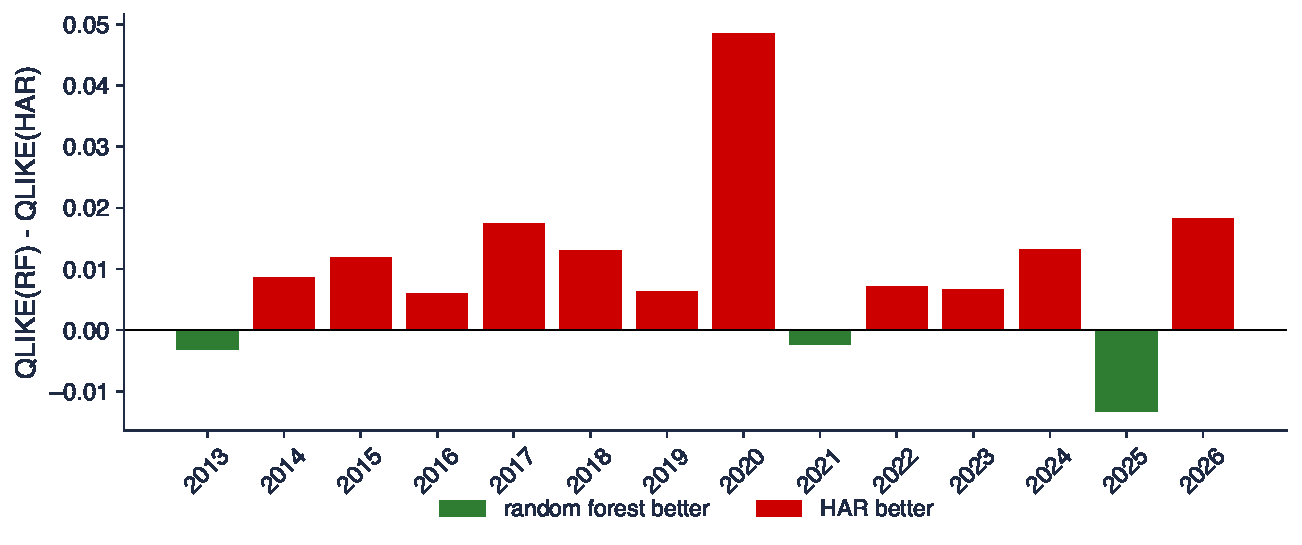
\includegraphics[width=0.96\textwidth,height=0.36\textheight,keepaspectratio]{ch13_sem_b1.pdf}
\end{center}
\vspace{-2mm}
\begin{itemize}
    \item 3\,448 days from 2 January 2013; $R^2_{OOS}$ against the mean: HAR $54.8\%$, forest $53.4\%$; forest against HAR: $-3.2\%$
    \item QLIKE: HAR $0.329$, forest $0.339$; DM $= +2.65$ (p 0.008); the forest is better in only 3 of 14 years
    \item Interpretation: no: with the same three features the forest is significantly worse than the linear HAR; the relation is close to linear in logs and the forest adds variance
\end{itemize}\sfmquantlet{Ch_13}{SFM_ch13_seminar}
\end{frame}

\begin{frame}{B2: Weekly Volatility of the DAX [Proposed]}
\itemsize{\footnotesize}
\begin{itemize}
\item \textbf{Question}: do lasso, random forest, gradient boosting or an MLP beat HAR for next week's DAX variance? Model: B1.
\item \textbf{Inputs}: DAX open, high, low and close since 2006; target: $\ln$ of the mean $v$ over the next 5 days; 11 features (HAR, 4 lags, quarter, $r_t$, $\min(r_t, 0)$, $|r_t|$)
\item \textbf{Tasks}
\begin{enumerate}
    \item Fit the five models walk-forward from 2012, purging the last 5 training days.
    \item Compute the out-of-sample $R^2$ against HAR and the mean QLIKE of each model.
    \item Run the Diebold--Mariano test of each model against HAR.
    \item Interpretation: which model would you use for the DAX?
\end{enumerate}
\item \textbf{Report}: one table and two sentences
\item Notebook: section B2
\end{itemize}
\end{frame}

\ifsolutions
\begin{frame}{B2: Solution [Proposed]}
\itemsize{\footnotesize}
\begin{center}
\footnotesize
\begin{tabular}{lrrrr}
\toprule
Model & $R^2_{OOS}$ vs.\ mean & $R^2_{OOS}$ vs.\ HAR & QLIKE & DM (p) \\
\midrule
HAR & $54.3$ & -- & $1.031$ & -- \\
Lasso & $57.9$ & ${+7.8}$ & $1.022$ & ${-2.51}$ (0.012) \\
RF & $56.9$ & ${+5.7}$ & $1.027$ & ${-0.76}$ (0.450) \\
GB & $55.0$ & ${+1.5}$ & $1.032$ & ${+0.18}$ (0.855) \\
MLP & $58.3$ & ${+8.7}$ & $1.022$ & ${-2.05}$ (0.040) \\
\bottomrule
\end{tabular}
\end{center}
\begin{itemize}
    \item 3\,727 days from 2 January 2012; $R^2_{OOS}$ in \%; DM against HAR, negative: better than HAR
    \item Interpretation: the lasso ($+7.8\%$, p 0.012) or the MLP ($+8.7\%$, p 0.040); the lasso is simpler and its gain is as large; trees do not beat HAR significantly
\end{itemize}\sfmquantlet{Ch_13}{SFM_ch13_seminar}
\end{frame}
\fi

\begin{frame}{B3: The Sign of DAX Returns [Solved]}
\itemsize{\footnotesize}
\begin{itemize}
\item \textbf{Question}: can a logit or a random forest predict whether the DAX rises tomorrow better than ``always up''?
\item \textbf{Inputs}: DAX closes since 2000; target $\mathbf{1}\{r_{t+1} > 0\}$; features: the last 5 returns, sums over 5, 21 and 63 days, volatility over 21 and 63 days
\item \textbf{Tasks}
\begin{enumerate}
    \item Fit both classifiers walk-forward from 2008, refitting each January.
    \item Compute the accuracy of each model and of the majority-class baseline.
    \item Test each accuracy against the baseline with the $z$ statistic, and compute the AUC.
    \item Draw the accuracy by year.
    \item Interpretation: does either model have skill?
\end{enumerate}
\item \textbf{Report}: six numbers, the chart and two sentences
\item Notebook: section B3
\end{itemize}
\end{frame}

\begin{frame}{B3: Solution [Solved]}
\itemsize{\scriptsize}
\begin{center}
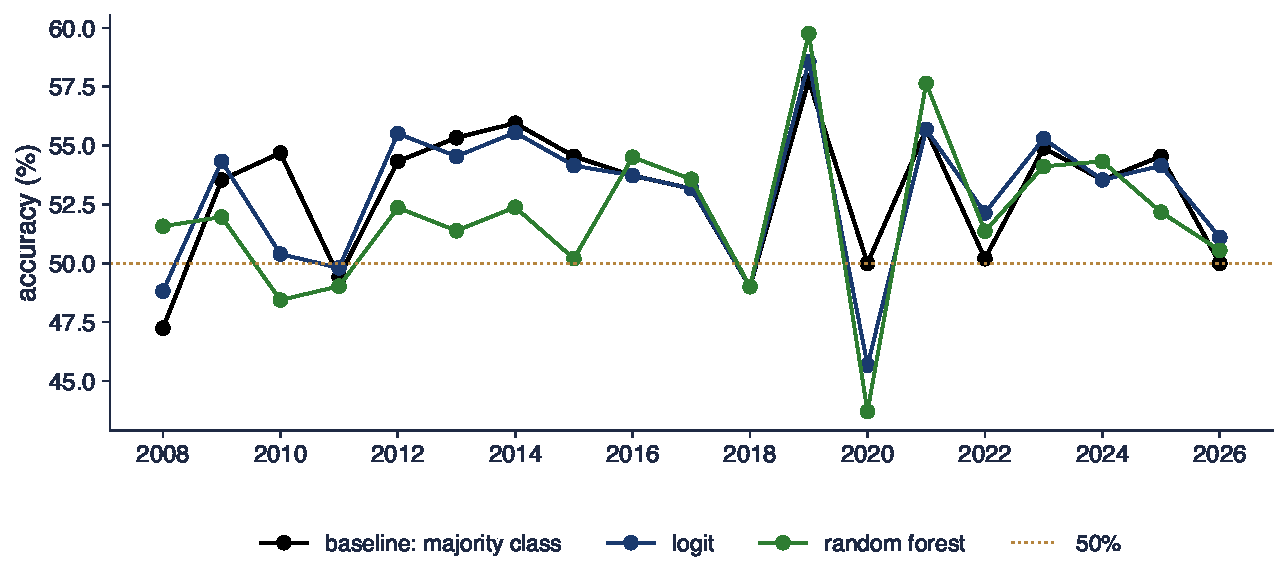
\includegraphics[width=0.96\textwidth,height=0.36\textheight,keepaspectratio]{ch13_sem_b3.pdf}
\end{center}
\vspace{-2mm}
\begin{itemize}
    \item $n = 4\,752$ days; up days 53.1\% = the baseline accuracy; logit 52.9\% ($z = -0.20$, p 0.839, AUC 0.507); forest 52.0\% ($z = -1.45$, p 0.146, AUC 0.508)
    \item The logit forecasts ``up'' on 90\% of the days; the forest beats the baseline in 8 of 19 years, as often as chance would allow
    \item Interpretation: no: both accuracies are at or below the baseline, and the AUC is close to 0.5; daily DAX returns are close to unpredictable (\sfmchlink{https://danpele.github.io/SFM/EN/Courses/chapter7_efficient_markets_random_walk_vr.pdf}{Chapter 7})
\end{itemize}\sfmquantlet{Ch_13}{SFM_ch13_seminar}
\end{frame}

\begin{frame}{B4: The Sign of Two BVB Stocks [Proposed]}
\itemsize{\footnotesize}
\begin{itemize}
\item \textbf{Question}: is the sign of Banca Transilvania and OMV Petrom returns easier to predict than that of the DAX? Model: B3.
\item \textbf{Inputs}: TLV (without 30--31 May 2016) and SNP adjusted closes since 2010; the features of B3; forecasts from 2014
\item \textbf{Tasks}
\begin{enumerate}
    \item Fit the logit, random forest and gradient boosting walk-forward from 2014.
    \item Compute the accuracy, the baseline accuracy, the $z$ statistic and the AUC for each stock and model.
    \item Interpretation: is there more predictability on the BVB than on the DAX?
\end{enumerate}
\item \textbf{Report}: one table and two sentences
\item Notebook: section B4
\end{itemize}
\end{frame}

\ifsolutions
\begin{frame}{B4: Solution [Proposed]}
\itemsize{\footnotesize}
\begin{center}
\footnotesize
\begin{tabular}{lrlrrr}
\toprule
& baseline (\%) & Model & accuracy (\%) & $z$ (p) & AUC \\
\midrule
TLV & 54.0 & Logit & 52.9 & ${-1.23}$ (0.219) & 0.488 \\
 &  & RF & 52.2 & ${-1.94}$ (0.053) & 0.509 \\
 &  & GB & 52.8 & ${-1.38}$ (0.168) & 0.506 \\
\midrule
SNP & 51.2 & Logit & 51.9 & ${+0.82}$ (0.414) & 0.509 \\
 &  & RF & 52.2 & ${+1.04}$ (0.299) & 0.509 \\
 &  & GB & 51.9 & ${+0.78}$ (0.436) & 0.513 \\
\bottomrule
\end{tabular}
\end{center}
\begin{itemize}
    \item TLV: 2\,902 days, SNP: 2\,905 days, from 2014
    \item Interpretation: no: no difference is significant at 5\%; SNP models are slightly above the baseline (forest $+1.0$ points, p 0.299), TLV models below it; AUC between 0.488 and 0.513
\end{itemize}\sfmquantlet{Ch_13}{SFM_ch13_seminar}
\end{frame}
\fi

\begin{frame}{B5: VaR 1\% of the DAX by Quantile Regression [Solved]}
\itemsize{\footnotesize}
\begin{itemize}
\item \textbf{Question}: does a linear quantile regression on volatility features give a better VaR 1\% than historical simulation?
\item \textbf{Inputs}: DAX since 2006; target $r_{t+1}$; features: $\sqrt{v_t}$, $\sqrt{\text{mean } v}$ over 5 and 22 days, $r_t$
\item \textbf{Tasks}
\begin{enumerate}
    \item Fit the 1\% quantile regression walk-forward from 2012 and set VaR 1\% $= -\hat q_{0.01}$.
    \item Compute the historical-simulation VaR 1\% on the last 500 days.
    \item Count the exceptions and run the Kupiec and Christoffersen tests; compute the average quantile loss.
    \item Draw both VaR forecasts in 2020--2022.
    \item Interpretation: which VaR would you report to a risk committee?
\end{enumerate}
\item \textbf{Report}: a table, the chart and two sentences
\item Notebook: section B5
\end{itemize}
\end{frame}

\begin{frame}{B5: Solution [Solved]}
\itemsize{\scriptsize}
\begin{center}
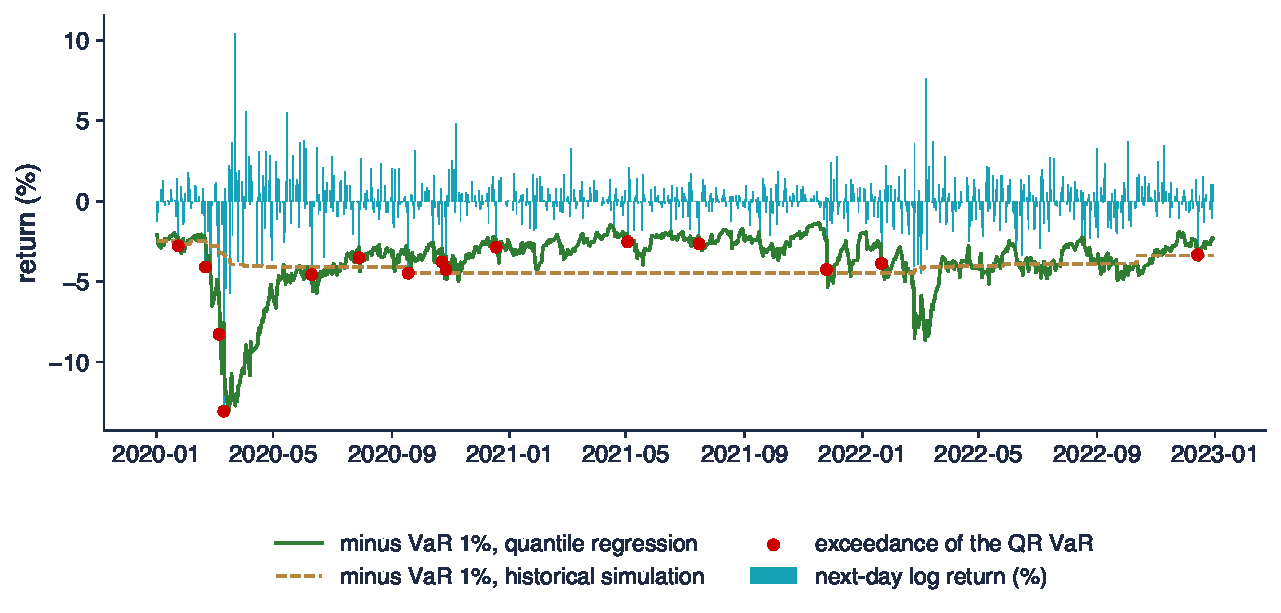
\includegraphics[width=0.96\textwidth,height=0.32\textheight,keepaspectratio]{ch13_sem_b5.pdf}
\end{center}
\vspace{-2mm}
\begin{center}
\scriptsize
\begin{tabular}{lrrrrr}
\toprule
Method & $x$ & rate (\%) & p Kupiec & p ind. & loss $\times 100$ \\
\midrule
QR & 39 & $1.05$ & 0.783 & 0.364 & $3.80$ \\
HS & 49 & $1.31$ & 0.066 & $<$\,0.001 & $4.75$ \\
\bottomrule
\end{tabular}
\end{center}
\begin{itemize}
    \item 3\,731 days from 2 January 2012; last fit: $\hat q_{0.01} = -0.472 -0.434\sqrt{v_t} -1.814\sqrt{v^{(w)}} -0.221\sqrt{v^{(m)}} +0.158 r_t$; VaR 1\% on 17 September 2026: 2.24\%
    \item Interpretation: the quantile regression: right rate, independent exceptions, smaller loss; HS is exceeded in clusters (13 times in 2020) because a 500-day window reacts slowly
\end{itemize}\sfmquantlet{Ch_13}{SFM_ch13_seminar}
\end{frame}

\begin{frame}{B6: Quantile Gradient Boosting for the DAX [Proposed]}
\itemsize{\footnotesize}
\begin{itemize}
\item \textbf{Question}: does a flexible quantile model improve on the linear quantile regression of B5? Model: B5.
\item \textbf{Inputs}: as in B5; gradient boosting with the quantile loss at 1\%, 300 trees of depth 2, learning rate 0.05, at least 50 days per leaf
\item \textbf{Tasks}
\begin{enumerate}
    \item Fit the quantile boosting walk-forward from 2012 and compute its VaR 1\%.
    \item Count the exceptions, run the Kupiec and Christoffersen tests and compute the quantile loss.
    \item Interpretation: is the flexible model worth it at the 1\% level?
\end{enumerate}
\item \textbf{Report}: one table and two sentences
\item Notebook: section B6
\end{itemize}
\end{frame}

\ifsolutions
\begin{frame}{B6: Solution [Proposed]}
\itemsize{\footnotesize}
\begin{center}
\footnotesize
\begin{tabular}{lrrrrrr}
\toprule
Method & $x$ & rate (\%) & p Kupiec & p ind. & loss $\times 100$ & mean VaR \\
\midrule
QR & 39 & $1.05$ & 0.783 & 0.364 & $3.80$ & $2.92$ \\
QGB & 71 & $1.90$ & $<$\,0.001 & 0.595 & $4.04$ & $2.71$ \\
\bottomrule
\end{tabular}
\end{center}
\begin{itemize}
    \item 3\,731 days; QGB: quantile gradient boosting
    \item Interpretation: no: boosting is exceeded far too often (1.90\%, p $<$\,0.001) and its loss is larger; at 1\% each leaf sees very few tail days, so the flexible model underestimates the risk
\end{itemize}\sfmquantlet{Ch_13}{SFM_ch13_seminar}
\end{frame}
\fi


%=============================================================================
\section{Part C: Open Questions and AI Critique}
%=============================================================================

\begin{frame}{C1: Does the S\&P 500 Help to Forecast BET Volatility? [Proposed]}
\itemsize{\footnotesize}
\begin{itemize}
\item \textbf{Question}: the BVB closes before New York; does yesterday's S\&P 500 volatility improve a HAR forecast of next week's BET variance?
\item \textbf{Inputs}: BET and S\&P 500 closes since 2008; proxy: squared daily returns (the BET has no high and low prices in our data); models: B1, B2
\item \textbf{Tasks}
\begin{enumerate}
    \item Build the HAR features of the BET and the HAR features of the S\&P 500 at the previous New York close.
    \item Compare HAR, HAR plus the S\&P 500 features (OLS) and a random forest on all features, walk-forward from 2012.
    \item Compute the out-of-sample $R^2$, QLIKE and the Diebold--Mariano tests against HAR.
    \item Interpretation: is the S\&P 500 information worth adding?
\end{enumerate}
\item \textbf{Report}: a table and a plan for a project
\item Notebook: section C1
\end{itemize}
\end{frame}

\ifsolutions
\begin{frame}{C1: Reference Analysis [Proposed]}
\itemsize{\footnotesize}
\begin{center}
\footnotesize
\begin{tabular}{lrrrr}
\toprule
Model & $R^2_{OOS}$ vs.\ mean & $R^2_{OOS}$ vs.\ HAR & QLIKE & DM (p) \\
\midrule
HAR & $40.7$ & -- & $0.782$ & -- \\
HAR+SPX & $41.4$ & ${+1.1}$ & $0.757$ & ${-1.57}$ (0.117) \\
RF+SPX & $38.8$ & ${-3.2}$ & $0.769$ & ${-0.93}$ (0.352) \\
\bottomrule
\end{tabular}
\end{center}
\begin{itemize}
    \item 3\,672 days from 4 January 2012; SPX: the S\&P 500 features of the previous New York close
    \item The S\&P 500 adds $+1.1\%$ to HAR and lowers QLIKE, but not significantly (p 0.117); the forest is worse than the linear model
    \item Project design: daily and monthly horizons, the DAX as a second external market, crisis periods separately, a range proxy for BVB stocks with high and low prices
\end{itemize}\sfmquantlet{Ch_13}{SFM_ch13_seminar}
\end{frame}
\fi

\begin{frame}{C2: Audit an AI Answer [Proposed]}
\itemsize{\scriptsize}
\begin{itemize}
    \item A student asked an AI assistant to summarise machine learning for the S\&P 500. The answer:
    \item \aiprompt{(a) With random 5-fold cross-validation a random forest explains 36.9\% of the next 21-day return: the market is predictable.}
    \item \aiprompt{(b) The forest fits next week's log variance better than HAR: in-sample R2 80.2\% against 73.7\%.}
    \item \aiprompt{(c) A forest predicts the sign of tomorrow's return correctly on 53.1\% of the days, more than a coin: it has skill.}
    \item \aiprompt{(d) For the VaR 99\% use quantile regression at tau = 0.99 on the next-day return.}
    \item \aiprompt{(e) The lasso removes the features whose t-statistics are not significant.}
    \item \aiprompt{(f) QLIKE punishes an under-forecast of the variance more than an over-forecast by the same factor.}
    \item Tasks
    \begin{itemize}
        \item 1. For each statement, say whether it is correct; if not, give the correct statement and, where possible, the correct number from the notebook (section C2).
        \item 2. Report: a list of six verdicts with one line of justification each.
    \end{itemize}
\end{itemize}
\end{frame}

\ifsolutions
\begin{frame}{C2: Solution [Proposed]}
\itemsize{\footnotesize}
\begin{itemize}
    \item (a) Wrong: overlapping targets leak through shuffled folds; walk-forward gives $R^2 = -38.0\%$, worse than the training mean
    \item (b) Wrong as evidence: an in-sample $R^2$ rewards flexibility; out of sample the forest gains only $+1.0\%$ over HAR (DM p 0.747)
    \item (c) Wrong: the baseline is ``always up'', right on 54.4\% of the days, not a coin; the forest is below it
    \item (d) Wrong twice: the level is the tail probability, VaR 1\%, and it needs $\tau = 0.01$ (the lower tail); VaR 1\% $= -\hat q_{0.01}$, a positive loss
    \item (e) Wrong: the lasso shrinks by a penalty; a zero coefficient is not a test, and the lasso gives no p-values
    \item (f) Correct: for a variance of 1, a forecast of 0.5 costs $1.307$ and a forecast of 2 costs $1.193$
\end{itemize}\sfmquantlet{Ch_13}{SFM_ch13_seminar}
\end{frame}
\fi


%=============================================================================
\section{Wrap-Up}
%=============================================================================

\begin{frame}{What You Should Take from Today}
\itemsize{\small}
\begin{itemize}
    \item The expected error is bias$^2$ + variance + noise: flexibility is not free
    \item Time series: walk-forward with purging; never shuffle days with overlapping targets
    \item Volatility: linear and penalised models are hard to beat; trees on the HAR features alone lose
    \item The sign of daily returns: compare with ``always up''; no model beats it here
    \item VaR 1\%: a linear quantile regression passes the backtests; a flexible quantile model at 1\% does not
    \item An AI answer is a draft: check the validation scheme, the baseline and the VaR convention
\end{itemize}
\end{frame}

\begin{frame}{After the Seminar}
\itemsize{\small}
\begin{itemize}
    \item Lecture 13 develops each topic of today: bias and variance, validation, ridge and lasso, trees and ensembles, neural networks, the three applications and data snooping
    \item Try the [Proposed] tasks in the notebook; the solutions are discussed in class
    \item C1 can grow into a team project: BVB stocks, external markets, several horizons
    \item Reading: \refISL, Ch.~2, 5, 6 and 8; \refFHH, Ch.~19
\end{itemize}
\end{frame}


%=============================================================================
\section{References}
%=============================================================================

\begin{frame}{References}
\itemsize{\tiny}
\begin{itemize}
    \item Christoffersen, P.F. (1998). \href{https://doi.org/10.2307/2527341}{Evaluating interval forecasts}. \textit{International Economic Review}, 39(4), 841--862.
    \item Corsi, F. (2009). \href{https://doi.org/10.1093/jjfinec/nbp001}{A simple approximate long-memory model of realized volatility}. \textit{Journal of Financial Econometrics}, 7(2), 174--196.
    \item Diebold, F.X., Mariano, R.S. (1995). \href{https://doi.org/10.1080/07350015.1995.10524599}{Comparing predictive accuracy}. \textit{Journal of Business \& Economic Statistics}, 13(3), 253--263.
    \item Franke, J., Härdle, W.K., Hafner, C.M. (2019). \href{https://doi.org/10.1007/978-3-030-13751-9}{\textit{Statistics of Financial Markets: An Introduction}}, 5th ed. Springer.
    \item Friedman, J.H. (2001). \href{https://doi.org/10.1214/aos/1013203451}{Greedy function approximation: a gradient boosting machine}. \textit{Annals of Statistics}, 29(5), 1189--1232.
    \item Hoerl, A.E., Kennard, R.W. (1970). \href{https://doi.org/10.1080/00401706.1970.10488634}{Ridge regression: biased estimation for nonorthogonal problems}. \textit{Technometrics}, 12(1), 55--67.
    \item James, G., Witten, D., Hastie, T., Tibshirani, R., Taylor, J. (2023). \href{https://doi.org/10.1007/978-3-031-38747-0}{\textit{An Introduction to Statistical Learning with Applications in Python}}. Springer.
    \item Koenker, R., Bassett, G. (1978). \href{https://doi.org/10.2307/1913643}{Regression quantiles}. \textit{Econometrica}, 46(1), 33--50.
    \item Kupiec, P.H. (1995). \href{https://doi.org/10.3905/jod.1995.407942}{Techniques for verifying the accuracy of risk measurement models}. \textit{Journal of Derivatives}, 3(2), 73--84.
    \item López de Prado, M. (2018). \href{https://www.wiley.com/en-us/Advances+in+Financial+Machine+Learning-p-9781119482086}{\textit{Advances in Financial Machine Learning}}. Wiley.
    \item Tibshirani, R. (1996). \href{https://doi.org/10.1111/j.2517-6161.1996.tb02080.x}{Regression shrinkage and selection via the lasso}. \textit{Journal of the Royal Statistical Society, Series B}, 58(1), 267--288.
\end{itemize}
\end{frame}

\end{document}
